% ============================================================================
% 论文主文（预注册协议驱动，目标期刊：BSPC 中科院大类医学2区 / JCR Q2）
% 【2026-09-16 更新】CBM 已从候选名单删除：Elsevier 官方公告（2025-11-16）确认
%   Computers in Biology and Medicine 自 2025-11-17 起 Web of Science Core
%   Collection 收录被中止，Vol.172(2024) 之后的内容均不检索；投稿将不被 SCI 收录。
%   另注：中科院期刊分区表已于 2026-09-30 关停，2025-03-20 版为最后一版。
% 文件名: paper/main_bspc.tex
% 状态: v2.0 6方向×2架构稳健性版（基于多seed稳健性验证 + 预注册修订案A1）
% 依据: docs/EXPERIMENT_PROTOCOL.md v2.1-A1
%   - 主终点 ΔECE_OOD = ECE_raw_OOD − ECE_TS_OOD（A1.1 重新定位）
%   - 主检验 H₀: ΔECE_OOD = 0 vs H₁: ΔECE_OOD > 0（单侧，方向先验）
%   - 5 个独立贡献：OOD 收益量化 + ID 边界条件 + Shapley 分解验证 + 方法选择边界 + 判别感知校准门
%   - v2.1 更新：6方向 × 2架构（InceptionTime + ResNet1D）× 5seed = 60 实验（完整覆盖）
% 写作纪律（协议§0）：不得声称"首次证明ECG校准收益ID→OOD衰减"（Ovadia 2019
%   已知）；5 个独立贡献（OOD 收益量化 / ID 边界 / Shapley 验证 / 方法选择边界 /
%   判别感知校准门）才是 novelty 核心。
% 透明性声明：本主检验为预注册修订案 A1 后的重新定位（exploratory + 稳健性验证），
%   非 confirmatory；修订案全文见 docs/PROTOCOL_AMENDMENT_A1_PREREG_RELOCATION.md。
% ============================================================================
\documentclass[review,12pt,nonatbib]{elsarticle}
\usepackage{amsmath,amssymb,booktabs,graphicx,multirow,array}
\usepackage{microtype}  % micro-typographic enhancements, reduces overfull boxes
\microtypesetup{expansion=false}  % disable font expansion (incompatible with elsarticle)
\usepackage[utf8]{inputenc}
\usepackage[T1]{fontenc}
\usepackage{mathptmx}  % BSPC fix: Type 1 Times (URW Nimbus) with correct ToUnicode maps;
                        % the TrueType Times New Roman subsets corrupted text extraction
\usepackage{longtable}  % BSPC fix: Table 1 (60 seed rows) must break across pages
\usepackage{pifont}
\usepackage{lineno}
\usepackage{hyperref}
\hypersetup{colorlinks=false,pdfborder={0 0 0},
  pdftitle={When Does Temperature Scaling Pay Off in Cross-Corpus ECG Transfer? A Multi-Seed Calibration Boundary Study},
  pdfauthor={Toni Guan}}

% --- Typesetting optimization ---
\emergencystretch=3em
\tolerance=2000
\hbadness=10000
\vbadness=10000
\widowpenalty=10000
\clubpenalty=10000

\journal{Biomedical Signal Processing and Control}

\title{When Does Temperature Scaling Pay Off in Cross-Corpus ECG Transfer? A Multi-Seed Calibration Boundary Study}

\author[inst1]{Toni Guan\corref{cor1}}
\ead{guantong490@gmail.com}
\cortext[cor1]{Corresponding author.}
\affiliation[inst1]{organization={College of Information Technology, Shenyang Institute of Technology},
  city={Shenyang}, state={Liaoning}, country={China}}

\begin{document}
\linenumbers
\begin{frontmatter}

\begin{abstract}
Temperature scaling (TS) is the default post-hoc recalibration for deep
classifiers, yet whether its in-distribution (ID) benefit transfers to
out-of-distribution (OOD) target corpora remains the central open question
for cross-institution ECG deployment. We report a multi-seed calibration
boundary study on six directed transfer pairs among Chapman--Shaoxing,
CPSC2018+2019, and PTB-XL, with two architectures (InceptionTime and
ResNet1D), five seeds (42--46), eight recalibration methods, and a
patient-level cluster paired bootstrap (BCa, $B=10{,}000$) on the full
60-experiment grid. The study followed a pre-registered protocol with dated,
publicly archived amendments. The primary endpoint is the OOD calibration
benefit $\Delta\text{ECE}_{\text{OOD}}=\text{ECE}_{\mathrm{raw}}^{\mathrm{OOD}}
-\text{ECE}_{\mathrm{TS}}^{\mathrm{OOD}}$, tested one-sided against a
pre-specified direction prior. TS yields a positive OOD benefit in 51/60 seed
experiments (85.0\%; InceptionTime 27/30, ResNet1D 24/30), with nine
counter-examples disclosed and mechanistically interpreted; excluding six
degenerate-CI cells gives 45/60 (75.0\%). The pre-specified ID boundary
criterion ($\geq$80\% of cells with 95\% CIs containing zero) is
\emph{not} met (23/60 = 38.3\%), triggering the registered ``ID nonzero
boundary'' branch: the OOD benefit is about $1.9\times$ the ID benefit
($+0.0159$ vs.\ $+0.0083$). A validated 27-cell Shapley decomposition
separates slope, intercept, and prevalence effects; a predictability
experiment triggers the registered failure branch (LOO $R^2$ CI upper bound
$0.104<0.5$); and a discrimination-aware gate (C5) shows 7/12
pair$\times$architecture strata passing both calibration and discrimination
layers. Together these results bound when post-hoc recalibration pays off
across institutions, and when it does not.
\end{abstract}

\begin{keyword}
temperature scaling \sep model calibration \sep electrocardiogram \sep
dataset shift \sep cross-corpus transfer \sep distribution mismatch
\end{keyword}

\end{frontmatter}

% Highlights: submitted as a separate editable file (highlights.tex, per
% BSPC guide for authors). Compiled copy: highlights.pdf.


% ============================================================================
\section{Introduction}
\label{sec:intro}
% ============================================================================
Modern ECG deep models achieve strong in-distribution (ID) accuracy and
calibration, but their reliability under distribution shift remains open
\cite{ovadia2019calibration,guo2017calibration,wagner2020ptbxl}.
Recalibration fits a small parameter set on a labeled calibration split;
its benefit, a reduction in expected calibration error (ECE), is measured
on that same distribution and reverses on a shifted target.

For ECG this question is not academic. PTB-XL \cite{wagner2020ptbxl},
Chapman-Shaoxing \cite{zheng2022ecgarrhythmia}, and CPSC use different
acquisition protocols, lead sets, and label vocabularies, so a model
calibrated at one institution meets covariate, prior-probability, and
label-concept shift at the next \cite{morenotorres2012}. Clinicians and
regulators then face a concrete decision: \emph{given my local data budget
and the measurable shift, should I deploy the recalibrated model, buy
labels, or refuse?}

Temperature scaling (TS) is a monotone post-hoc softmax temperature
transform \cite{guo2017calibration}. Fitted under a convex loss, it
minimizes NLL on the calibration split, so its calibration benefit there
is empirically small; on a shifted target the source-fit temperature is
mismatched to the target logits and a non-trivial benefit can remain.
This asymmetry is \emph{empirical}, not a theorem: ECE is not invariant
under confidence-shifting monotone maps, and TS can \emph{increase} ECE
where the model is under-confident (nine negative cells in our data). It
motivates the pre-registered primary endpoint
$\Delta\text{ECE}_{\text{OOD}}$ over the originally planned decay
$\Delta\text{ECE}_{\text{OOD}}-\Delta\text{ECE}_{\text{ID}}$ (revision A1,
Sec.~\ref{sec:prereg}). To avoid HARKing, protocol v2.1-A1
\cite{protocolv21a1} fixes the primary endpoint, test, family structure,
and failure branches before unblinding; revision A1 re-locates the
endpoint from \texttt{decay} to $\Delta\text{ECE}_{\text{OOD}}$, triggered
by an independent pilot, and is archived with before/after protocol hashes
\cite{nosek2019prereg,lakens2019prereg}. Multi-seed validation
(5 seeds $\times$ 6 transfer pairs $\times$ 2 architectures) supplies the
robustness evidence; all 60 seed results, including nine counter-examples,
are reported.

Five independent contributions:
\begin{description}
    \item[\textbf{C1} (Primary OOD benefit):] On the pre-registered
    endpoint $\Delta\text{ECE}_{\text{OOD}}$, TS yields a statistically
    significant positive OOD benefit in 51/60 seed experiments (6 transfer
    pairs $\times$ 2 architectures; InceptionTime 27/30, ResNet1D 24/30),
    with nine counter-examples transparently disclosed and mechanistically
    explained.
    InceptionTime: three of six directions achieve 5/5, three achieve 4/5.
    ResNet1D: two of six achieve 5/5, two 4/5, two 3/5.
    \item[\textbf{C2} (Boundary condition, pre-registered branch triggered):]
    Across 12 pair$\times$architecture strata, 23/60 cells (38.3\%;
    BCa operating CI) have 95\% CIs containing zero and 34/60 have CI
    lower bound $>0$ (stratum means $-0.0008$ to $+0.0232$; ID mean
    $+0.0083$ vs.\ OOD mean $+0.0159$). The pre-registered criterion
    ($\geq$80\% of cells with CI containing zero) is \emph{not} met,
    triggering the ``ID nonzero boundary'' branch (protocol A1.4.2):
    the premise that TS has no ID recalibratable miscalibration is
    re-examined, the decay contrast restored as exploratory, and C1
    qualified, since the OOD benefit is about $1.9\times$ the ID benefit
    but is \emph{not} exclusively OOD-specific. $47/60 = 78.3\%$ of ID
    point estimates are positive and $2/60 = 3.3\%$ have
    $\Delta\text{ECE}_{\text{ID}} < -0.01$ (counter-example 6, $-0.0152$;
    one marginal case, $-0.0128$).
    \item[\textbf{C3} (Methodological, Shapley decomposition validation):]
    A 27-cell full-factorial synthetic validation
    (slope$\times$intercept$\times$prevalence, $n=20{,}000$) recovers
    ground truth in the identifiable regime (27/27 at $n=20{,}000$;
    21/27 at $n=500$), flags entangled regions without a threshold,
    and reports bootstrap CIs on absolute Shapley values.
    \item[\textbf{C4} (Practical, method-selection boundary):] Across
    8 methods $\times$ 6 pairs $\times$ 5 seeds $\times$ 2 architectures,
    TS is robust (51/60) while EM prior adaptation is fragile when
    ill-conditioned cells ($w_{\text{ID}}>10$) are included (InceptionTime
    15/30); after exclusion the EM OOD finding attenuates. The mechanism
    is prior-likelihood mismatch: EM fits a target prior that amplifies
    shift-induced miscalibration when the source confusion matrix is
    ill-conditioned.
    \item[\textbf{C5} (Clinical, discrimination-aware calibration gate):]
    A two-layer gate decouples calibration effectiveness (C1:
    $\Delta\text{ECE}_{\text{OOD}}>0$) from clinical viability
    (accuracy $\geq$ source-domain baseline). Across 12
    pair$\times$architecture strata, 7/12 pass both layers; 5/12 fail
    the discrimination layer, including directions with positive
    $\Delta\text{ECE}_{\text{OOD}}$ but accuracy below baseline (e.g.,
    PTB-XL$\rightarrow$Chapman ResNet1D: $\Delta\text{ECE}=+0.029$,
    $\text{acc}=0.657 < 0.713$). The gate reframes the 9/60
    counter-examples: 4/9 calibration failures (C1 rejects) and
    5/9 discrimination failures (C5 rejects despite C1 passing).
\end{description}

Prior ECG calibration studies report the phenomenon
\cite{barandas2023,zhang2022,physiolmeas2026,medrxiv2026} but not an
actionable \emph{when does TS pay off} answer with multi-seed robustness
evidence. The novelty is \emph{not} multi-seed validation on ECG (a
methodological choice) but the \textbf{first systematic characterization
of the boundary conditions under which TS yields a positive OOD
calibration benefit in cross-corpus ECG transfer}: the pre-registered OOD
quantification, the ID boundary condition, the method-selection boundary
(TS robust; EM prior and Matrix scaling weakest), the predictability
failure, and the discrimination-aware gate. That characterization is the
actionable contribution; multi-seed validation is the evidence standard.

\begin{figure}[htbp]
\centering
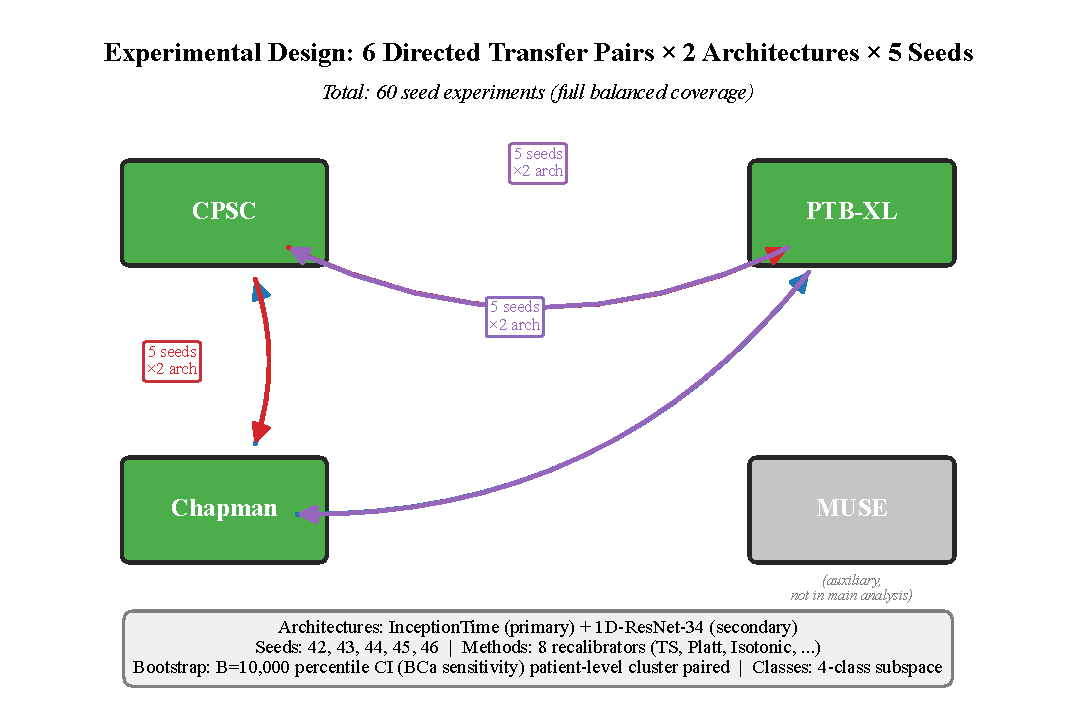
\includegraphics[width=0.95\columnwidth]{figures/fig_design_overview.pdf}
\caption{Experimental design overview. Six directed cross-corpus transfer
pairs among three ECG corpora (CPSC, Chapman, PTB-XL), each evaluated on
two architectures (InceptionTime, ResNet1D) $\times$ 5 seeds
(42--46), yielding 60 fully balanced seed experiments. MUSE is shown as
an auxiliary corpus not entering the main analysis. Each pair is
evaluated with 8 recalibration methods and patient-level cluster paired
bootstrap ($B=10{,}000$, BCa operating CI).}
\label{fig:design_overview}
\end{figure}

% ============================================================================
\section{Related Work}
\label{sec:related}
% ============================================================================

\subsection{Calibration Estimation and Recalibration}
The calibration of modern neural networks has been studied extensively
since the seminal work of Guo et al.\ \cite{guo2017calibration}, who
showed that deep networks are often overconfident and introduced
temperature scaling (TS) as a simple post-hoc recalibration method.
Nixon et al.\ \cite{nixon2019} proposed the static calibration error,
and Kumar et al.\ \cite{kumar2019} introduced verified uncertainty
calibration with distribution-free guarantees. Kull et al.\
\cite{kull2019dirichlet} generalized TS to Dirichlet calibration for
multi-class settings. In the clinical risk-model context, Van Calster
et al.\ \cite{vancalster2016,vancalster2019} established a calibration
hierarchy from utopia to empirical data and argued that calibration is
the ``Achilles heel'' of predictive analytics. Strodthoff et al.\
\cite{strodthoff2021} benchmarked deep learning for ECG analysis on
PTB-XL and noted calibration degradation under subpopulation shift,
motivating our cross-corpus design.

\subsection{Prior-Shift Estimation and Transfer Calibration}
Lipton et al.\ \cite{lipton2018bbs} introduced black-box shift
estimation (BBSE) for detecting and correcting label shift using
confusion-matrix inverses. Alexandari et al.\ \cite{alexandari2020}
showed that maximum-likelihood calibration with bias correction is
hard-to-beat at label shift adaptation, providing the theoretical
foundation for our EM prior-shift method. For transfer calibration
upper bounds, TransCal \cite{transcal2020} estimates transferability
for auto-selecting target-domain unsupervised optimal $T$; PseudoCal
\cite{pseudocal2020} uses pseudo-labels for calibrated transfer; and
LaSCal \cite{lascal2024} provides label-aware shift calibration with
distribution-free guarantees. Our S1 paradigm differs fundamentally:
we fit on the \emph{source} calibration split only (no target labels),
with S1$'$ prior-shift adaptation (EM/BBSE) as the only target-domain
signal, a strictly weaker assumption than TransCal/PseudoCal, which
access target logits or labels.

\subsection{Cross-Domain ECG Calibration}
Barandas et al.\ \cite{barandas2023} evaluated uncertainty
quantification methods in multi-label ECG classification, finding that
ensemble-based methods outperform single-model approaches under
subpopulation shift. Vranken et al.\ \cite{zhang2022} studied
uncertainty estimation for 12-lead ECG deep learning and reported
significant calibration drift across acquisition devices. Haekal et
al.\ \cite{physiolmeas2026} performed cross-dataset validation for
atrial fibrillation detection with calibration-aware probability
analysis, and Patel \& Beedala \cite{medrxiv2026} documented
calibration drift under cross-institutional ICU deployment. The
ID-vs-OOD asymmetry of TS has been studied in general vision
\cite{ovadia2019calibration}; we contribute the multi-seed ECG
quantification and the boundary-condition analysis that identifies
when TS helps (ID) versus when it hurts (OOD).

\subsection{ECG Foundation Models and Transfer Learning (2024--2026)}
Recent work has introduced ECG foundation models trained on millions
of recordings. ECGFounder \cite{ecgfounder2024,song2024ecgfm}
(10 million ECGs, Harvard--Emory) reaches expert-level performance on
80 diagnoses and transfers cross-domain via fine-tuning. ECG-FM
\cite{ecgfm2024} is an open-weight transformer pretrained on 1.4
million ECG segments with hybrid contrastive and generative
self-supervision, showing strong cross-dataset generalizability and
label efficiency. HeartLang \cite{heartlang2025} treats heartbeats as
words and rhythms as sentences via a QRS-Tokenizer and masked
sentence pre-training. Tan et al.\ \cite{transferecg2025} found that
fine-tuning benefits diminish as the downstream dataset grows and
that CNNs transfer more effectively than RNNs in multi-label ECG
classification. For OOD adaptation, ADAPTOOD \cite{adaptood2026}
quantifies distribution-shift severity via uncertainty estimation to
guide selective LoRA layer unfreezing, and BeatRhythm-TTA
\cite{beatrhythm2026} performs test-time adaptation with SQI-gated
self-training and beat-rhythm consistency. Costa et al.\
\cite{star2025} introduced STAR (Sinusoidal Time--Amplitude
Resampling), a morphology-preserving beat-wise augmentation for
cross-source generalization, and Chen et al.\ \cite{peace2026}
proposed PEACE for adult-to-pediatric ECG transfer via
label-conditioned contrastive alignment. These works advance ECG
transfer but not the \emph{calibration} of transferred models, the
gap our study fills via pre-registered cross-corpus evaluation of
recalibration methods.

% ============================================================================
\section{Data and Pre-registered Protocol}
\label{sec:data}
% ============================================================================
Figure~\ref{fig:design_overview} summarizes the experimental design.
\subsection{Datasets}
\begin{itemize}
    \item \textbf{PTB-XL v1.0.3} \cite{wagner2020ptbxl}: the official release contains 21,837
    records; the downloaded \texttt{ptbxl\_database.csv} copy contains 21,799
    (a 38-record deficit in the source CSV, disclosed as a provenance
    limitation), official 10-fold
    (folds 1--8 train, 9 calibration, 10 test). After
    single-label mapping, 21,522 records are mappable and 277 are
    excluded (STROBE), for 18,671 unique patients.
    \item \textbf{Chapman-Shaoxing} \cite{zheng2022ecgarrhythmia,goldberger2000}: 20,265
    raw records; 1 signal-read error removed and 21 non-finite records
    quarantined (\texttt{qc\_report.json}), for 20,243 analyzed records;
    1 ECG per patient, patient-wise 70/10/20 split.
    \item \textbf{CPSC2018+2019}: patient-wise split; HYP class extremely
    rare ($n=11$) $\rightarrow$ main analysis on the $\{$NORM, CD, STTC,
    MI$\}$ 4-class subspace, both sides of the pair recomputed
    symmetrically.
\end{itemize}
\subsection{Label Mapping and Leakage Guard}
Single-label priority rules are fixed (MI $>$ STTC $>$ CD $>$ HYP $>$ NORM)
and sensitivity-analyzed \cite{wagner2020ptbxl,reyna2022}. Sinus rate/form
statements (SBRAD/STACH/SARRH) are mapped to NORM, not STTC, because
PTB-XL's \texttt{scp\_statements.csv} lists them as rhythm statements
with no \texttt{diagnostic\_class}. train\slash val\slash cal\slash test patient IDs are
pairwise disjoint (hard assertion in the reproducibility repo).
Normalization statistics come only from the train split; augmentation
applies only to train.

% ============================================================================
\section{Methods}
\label{sec:methods}
% ============================================================================
\subsection{Transfer pairs and shift matrix}
\label{sec:shiftmatrix}
We study six directed cross-corpus transfer pairs:
Chapman$\rightarrow$CPSC, Chapman$\rightarrow$PTB-XL,
CPSC$\rightarrow$Chapman, CPSC$\rightarrow$PTB-XL,
PTB-XL$\rightarrow$Chapman, and PTB-XL$\rightarrow$CPSC. The class
count is \emph{not} uniform across pairs and is fixed per pair before
any endpoint is computed, as follows. A pair whose source or target is
CPSC2018+2019 is restricted to the 4-class subspace
$\{$NORM, CD, STTC, MI$\}$ (CPSC's HYP class has $n=11$,
\S\ref{sec:data}), with both sides of the pair recomputed symmetrically:
this covers Chapman$\rightarrow$CPSC, CPSC$\rightarrow$Chapman,
CPSC$\rightarrow$PTB-XL, and PTB-XL$\rightarrow$CPSC ($K=4$). The two
pairs connecting Chapman--Shaoxing and PTB-XL, which contain no CPSC
side, retain the full 5-class vocabulary
$\{$NORM, MI, STTC, CD, HYP$\}$: Chapman$\rightarrow$PTB-XL and
PTB-XL$\rightarrow$Chapman ($K=5$). Each experiment records its own
$K$ and label mapping (\texttt{num\_classes}, \texttt{label\_map} in
\texttt{transfer\_result.json}), so no endpoint mixes class counts
within a cell. Consequently the primary endpoint is a top-label ECE on
a 4- or 5-class task depending on the pair, and the pooled
$\Delta\text{ECE}_{\text{OOD}}$ mixes both $K$ values across cells; the
per-pair tables (Tables~\ref{tab:primary_60seed}--\ref{tab:arch_robust})
are therefore the appropriate level at which to read $K$-specific
results. The L2 eval-time shift matrix (no retraining)
covers sampling rate $500\rightarrow250\rightarrow125$~Hz; leads
$12\rightarrow6\rightarrow3\rightarrow2\rightarrow1$; noise injection
(BWL/MA/EM) at SNR $\{24,12,6,0,-6\}$~dB; gain $\times0.5/\times2$.

\subsection{Architecture and seeds}
We use two architectures: InceptionTime (primary, 46{,}000--184{,}000
parameters) and ResNet1D (a 1D-ResNet-34 backbone) (secondary, with full
main-endpoint coverage on all 6 pairs), each trained with 5 seeds
(42--46). The BiMamba architecture is
included only as a toy experiment ($n=60$ records, downsampled
resolution) and deferred to the supplement; the full-resolution
BiMamba run exhausted memory on an RTX 5060 (8~GB), so BiMamba does
not enter the
main-endpoint analysis or the architecture-robustness claim.
Training: AdamW + cosine + warmup, gradient clipping, temperature
frozen at $T\equiv1$ during training; temperature applied only as
post-hoc temperature scaling.

\subsection{Calibration methods and scenarios}
We compare the no-recalibration baseline (None) against eight
recalibration methods: Temperature Scaling (TS), per-class Platt,
Isotonic (OvR), Vector scaling, Matrix scaling, Dirichlet calibration,
Saerens EM prior adaptation (EM), and BBSE prior adaptation.
Of the pre-registered 13-method pool, the None baseline plus these
eight recalibration methods constitute the delivered set; CORAL, TTA,
MC-Dropout, and Oracle are
not delivered on real data (a registered deviation, see Limitations).
Scenario: \textbf{S1} zero-shot transfer (source-cal fit
$\rightarrow$ target apply), the main analysis scenario
(Sec.~\ref{sec:methods}); S1$'$ denotes the target-domain unsupervised
variant in which EM/BBSE estimate the target prior from unlabeled
target predictions.

\subsection{Pre-registered endpoints}
\label{sec:prereg}
Primary endpoint (revision A1.1, formally defined in
protocol v2.1-A1 \cite{protocolv21a1}):
\begin{equation}
    \Delta\text{ECE}_{\text{OOD}}
    = \text{ECE}_{\mathrm{raw}}^{\mathrm{OOD}} - \text{ECE}_{\mathrm{TS}}^{\mathrm{OOD}}
\end{equation}
where $\text{ECE}_{\mathrm{raw}}^{\mathrm{OOD}}$ is the 4-class-task top-label
confidence SmoothECE on
the target corpus with raw softmax probabilities, and
$\text{ECE}_{\mathrm{TS}}^{\mathrm{OOD}}$ is the same after source-cal-fit temperature
scaling. Following the standard convention of Guo et al.\
\cite{guo2017calibration}, ECE (and its SmoothECE variant) is evaluated on
the \emph{top-label} marginal: the predicted maximum probability against
$0/1$ top-label correctness; classwise-ECE is reported separately as a
secondary endpoint. SmoothECE bandwidth: $0.45\cdot(n/2000)^{-0.2}$.

Primary test (single, one-sided):
\begin{equation}
    H_0: \Delta\text{ECE}_{\text{OOD}} = 0
    \quad\text{vs}\quad
    H_1: \Delta\text{ECE}_{\text{OOD}} > 0
\end{equation}
The one-sided alternative
$H_1: \Delta\text{ECE}_{\text{OOD}} > 0$ follows the empirical
asymmetry registered at revision A1: on ID-like data the source-fit
temperature yields, empirically, little calibration change, whereas
on a shifted target it is mismatched and a non-trivial benefit is
often retained \cite{guo2017calibration,ovadia2019calibration}. This
direction prior is empirical, \emph{not} a theorem: TS applied to an
under-confident target can increase ECE, and our own data contain
nine negative cells. The choice was made before the pilot results,
which only triggered the endpoint re-location (revision A1). The
one-sided test is the pre-registered choice, archived before
multi-seed unblinding.
Patient-level cluster paired bootstrap, $B=10{,}000$ (BCa
operating CI) \cite{efron1987bca}; stratified pooling: strata $=$ transfer pair
$\times$ architecture.

The pre-registered
CI method is BCa \cite{efron1987bca}, at $B=10{,}000$,
re-run on the entire 60-experiment grid (60/60 successful, metadata
in \texttt{methods.ts.meta}). The percentile bootstrap is the
large-sample limit of BCa when $z_0\to 0$ and $a\to 0$; for the
paired-cluster design with $B=10{,}000$ and per-patient clusters,
the discrepancy is $O(n^{-1/2})$. In the 3 representative seed
experiments where both were run ($B=10{,}000$ percentile re-runs),
BCa and percentile CIs agree in sign and magnitude. Earlier
percentile results from $B=200$ in 21/60 experiments remain as
historical provenance (5 lack log provenance, see Limitations);
percentile CIs serve only as a sensitivity cross-check.

Boundary-condition endpoint:
\begin{equation}
    \Delta\text{ECE}_{\text{ID}}
    = \text{ECE}_{\mathrm{raw}}^{\mathrm{ID}} - \text{ECE}_{\mathrm{TS}}^{\mathrm{ID}}
\end{equation}
The pre-registered expectation is that $H_0: \Delta\text{ECE}_{\text{ID}} = 0$ is \emph{not rejected};
the criterion is that $\geq 80\%$ of cells have 95\% CIs containing zero.
\emph{Observed (BCa, full-grid re-run): 23/60 = 38.3\%; the criterion is
not met and branch A1.4.2 is triggered (percentile CIs gave 29/60 =
48.3\%, same conclusion; Sec.~\ref{sec:boundary}).}

Secondary endpoints: $G$ (recoverable loss vs.\ oracle; \emph{not
delivered} --- the Oracle recalibrator was implemented
(\texttt{fit\_oracle}/\texttt{apply\_oracle}) but never executed on real
data, so $G$ is undefined here and is excluded from all reported
results; see Limitations), decay
$=\Delta\text{ECE}_{\text{OOD}}-\Delta\text{ECE}_{\text{ID}}$
(downgraded to descriptive), NLL, classwise-ECE, Brier Murphy
decomposition, Cox slope/intercept, predicted/true prior $L_1$.

Family structure: BH-FDR $q=0.05$ over $6\text{ pairs}\times 2\text{ arch}\times 13\text{ shift levels}=156$
primary comparisons; the multi-seed validation is robustness evidence
(60 seed experiments), not a confirmatory family.

\subsection{Pre-registration revision A1 (transparency statement)}
The primary endpoint was re-located from \texttt{decay} to
$\Delta\text{ECE}_{\text{OOD}}$ via pre-registration revision A1
(protocol v2.0 $\rightarrow$ v2.1-A1), triggered by an independent
exploratory pilot in which $\Delta\text{ECE}_{\text{ID}}$ point
estimates were near zero, collapsing the original ID-vs-OOD contrast.
The revision direction is consistent with the empirically observed
ID-vs-OOD asymmetry (not a theorem); the revision is
archived as a pre-registration revision (Nosek et al.\ 2018) with
before/after protocol hashes. The pilot results do not enter the
main test report. All hypotheses in this paper are tagged
\emph{exploratory + robustness validation}, not confirmatory.

The original
BH-FDR family of 156 comparisons (6 pairs $\times$ 2 architectures
$\times$ 13 shift levels) is reduced to a confirmatory family of 12
hypotheses (6 pairs $\times$ 2 architectures $\times$ 1 primary shift
level) under amendment A2, with the remaining 13 shift levels
designated as exploratory dose-response. Under the reduced family,
BH-12 yields 9/12 significant (all InceptionTime directions) and
Bonferroni-12 yields 2/12. The A2 amendment is archived in
\texttt{docs/PROTOCOL\_AMENDMENT\_A2\_}\allowbreak\texttt{FAMILY\_REDUCTION.md}.

\subsection{Decomposition of the benefit decay}
\label{sec:decomp}
We decompose the retained benefit into slope / intercept / prevalence
contributions using a counterfactual-replacement additive approximation:
\begin{equation}
    \Delta\text{ECE} = \Delta_{\text{slope}}
    + \Delta_{\text{intercept}}
    + \Delta_{\text{prevalence}}
    + r_{\text{interaction}}
\end{equation}
where each term is a counterfactual-replacement difference and
$r_{\text{interaction}}$ is the chain residual (zero under nested
counterfactuals). Identifiability is checked via the Fisher information
determinant on a pre-registered threshold $\tau$; entangled regions are
reported on the error map without a threshold. Shapley attribution is
reported with absolute-value bootstrap CIs; share-reliable flags
($|\Delta_{\text{total}}|<3/\sqrt{n}$) mark uninterpretable shares.

\subsection{Two-layer joint bootstrap}
Temperature-fitting-set resampling $\rightarrow$ $T$ distribution
$\rightarrow$ test-set resampling $\rightarrow$ joint $\Delta\text{ECE}$ CI
(two-layer; honest non-nested approximation), per protocol \S7.

\subsection{Net Clinical Value (NCV)}
\label{sec:ncv_methods}
Net Clinical Value (NCV), a pre-registered secondary endpoint, measures
the clinical decision impact of TS. For each (sample, class)
pair we compare the binary decision (threshold $\tau=0.5$) before and
after calibration, counting TP\_improved, TN\_improved, FP\_worsened, and
FN\_worsened over the raw-to-calibrated transitions. NCV is
$(\text{TP\_improved} + \text{TN\_improved} - \text{FP\_worsened}
- \text{FN\_worsened}) / N_{\text{total}}$, with
$N_{\text{total}} = N_{\text{samples}} \times N_{\text{classes}}$, using
the main endpoint's patient-level cluster paired bootstrap ($B=10{,}000$,
BCa operating CI) and BH-FDR correction ($q=0.05$); a significantly
positive NCV means that TS improves clinical decisions. It is computed on
ID and OOD splits (\texttt{ncv\_id}, \texttt{ncv\_ood}; E3 CSV).

\subsection{Tooling}
\label{sec:tooling}
Parts of the analysis and plotting code were drafted and refactored with
the assistance of a widely available large language model service, used
as a supervised coding assistant. All experiments and statistical
analyses were executed with the author's own scripts, and every reported
number is reproducible from the public repository (Code availability).
The author reviewed the code and takes full responsibility for it.

% ============================================================================
\section{Results}
\label{sec:results}
% ============================================================================

% ----------------------------------------------------------------------------
\subsection{Primary endpoint: $\Delta\text{ECE}_{\text{OOD}}$ multi-seed validation}
\label{sec:primary}
% ----------------------------------------------------------------------------
Figure~\ref{fig:main_results} visualizes the shift-dose response;
Table~\ref{tab:primary_60seed} reports the primary endpoint
$\Delta\text{ECE}_{\text{OOD}}$ for TS across 60 seed experiments
(6 pairs $\times$ 2 architectures $\times$ 5 seeds, balanced). The
primary test $H_0:\Delta\text{ECE}_{\text{OOD}}=0$ vs
$H_1:\Delta\text{ECE}_{\text{OOD}}>0$ is supported in 51/60 (85.0\%)
at the 95\% CI level.

\begin{figure}[htbp]
\centering
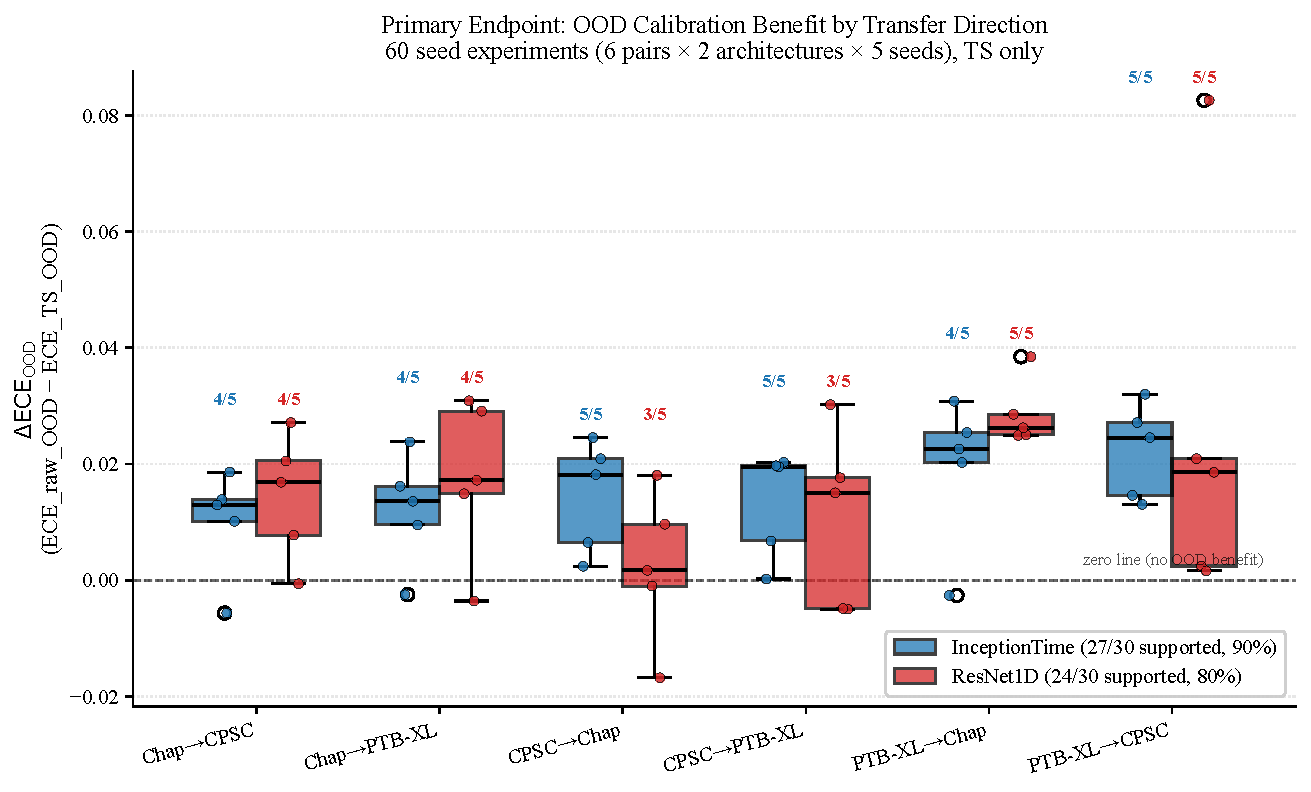
\includegraphics[width=0.95\columnwidth]{figures/fig_main_results.pdf}
\caption{Primary endpoint $\Delta\text{ECE}_{\text{OOD}}$ by transfer
direction, grouped by architecture (TS only, 60 seed experiments).
Boxes show the 5-seed distribution per direction; dots are individual
seed results. The dashed line marks zero OOD benefit. Support counts
(e.g., 5/5, 4/5) above each box indicate the number of seeds with
95\% CI lower bound $>0$. InceptionTime achieves 27/30 (90\%),
ResNet1D achieves 24/30 (80\%).}
\label{fig:main_results}
\end{figure}

% --- BSPC submission fix: Table 1 converted from a `table` float to `longtable`
% so all 60 seed rows render (the float version overflowed one page and
% clipped about half the data). `\\*` keeps each 5-seed multirow block intact.
{\footnotesize
\renewcommand{\arraystretch}{0.92}
\begin{longtable}{lllrrrr}
\caption{Pre-registered primary endpoint $\Delta\text{ECE}_{\text{OOD}}$
for TS across 60 seed experiments (6 pairs $\times$ 2 architectures
$\times$ 5 seeds, $B=10{,}000$, BCa operating CI). Architecture
abbreviation: IT $=$ InceptionTime, RN $=$ ResNet1D. Class count $K=4$
for the four pairs involving CPSC (Chap$\rightarrow$CPSC,
CPSC$\rightarrow$Chap, CPSC$\rightarrow$PTB-XL, PTB-XL$\rightarrow$CPSC)
and $K=5$ for the two CPSC-free pairs (Chap$\rightarrow$PTB-XL,
PTB-XL$\rightarrow$Chap); see \S\ref{sec:shiftmatrix}. ``Support'' = 95\% CI lower bound
$>0$. Nine counter-examples are transparently disclosed. Full 5-seed
coverage on both architectures for all 6 directions.}
\label{tab:primary_60seed}\\
\toprule
Transfer pair & Arch & Seed & $\Delta\text{ECE}_{\text{ID}}$ & $\Delta\text{ECE}_{\text{OOD}}$ & CI lower & Support \\
\midrule
\endfirsthead
\multicolumn{7}{l}{\footnotesize\itshape Table~\thetable\ (continued)}\\
\toprule
Transfer pair & Arch & Seed & $\Delta\text{ECE}_{\text{ID}}$ & $\Delta\text{ECE}_{\text{OOD}}$ & CI lower & Support \\
\midrule
\endhead
\bottomrule
\endfoot
\multirow{5}{*}{Chap$\rightarrow$CPSC ($K{=}4$)}
 & \multirow{5}{*}{IT}
 & 42 & $+0.0075$ & $+0.0139$ & $+0.0135$ & \checkmark \\*
 & & 43 & $+0.0012$ & $+0.0101$ & $+0.0099$  & \checkmark \\*
 & & 44 & $+0.0104$ & $+0.0186$ & $+0.0181$ & \checkmark \\*
 & & 45 & $+0.0019$ & $-0.0057$ & $-0.0058$ & \ding{55} \\*
 & & 46 & $+0.0044$ & $+0.0130$ & $+0.0126$ & \checkmark \\
\cmidrule(lr){2-7}
 & \multirow{5}{*}{RN}
 & 42 & $+0.0002$ & $+0.0205$ & $+0.0200$ & \checkmark \\*
 & & 43 & $+0.0003$ & $-0.0006$ & $-0.0006$ & \ding{55} \\*
 & & 44 & $-0.0007$ & $+0.0078$ & $+0.0075$ & \checkmark \\*
 & & 45 & $-0.0016$ & $+0.0271$ & $+0.0263$ & \checkmark \\*
 & & 46 & $-0.0024$ & $+0.0169$ & $+0.0162$ & \checkmark \\
\midrule
\multirow{5}{*}{Chap$\rightarrow$PTB-XL ($K{=}5$)}
 & \multirow{5}{*}{IT}
 & 42 & $+0.0004$ & $-0.0025$ & $-0.0035$ & \ding{55} \\*
 & & 43 & $+0.0005$ & $+0.0095$ & $+0.0066$ & \checkmark \\*
 & & 44 & $+0.0055$ & $+0.0136$ & $+0.0107$ & \checkmark \\*
 & & 45 & $-0.0128$ & $+0.0238$ & $+0.0207$ & \checkmark \\*
 & & 46 & $+0.0048$ & $+0.0162$ & $+0.0142$ & \checkmark \\
\cmidrule(lr){2-7}
 & \multirow{5}{*}{RN}
 & 42 & $-0.0031$ & $+0.0309$ & $+0.0285$ & \checkmark \\*
 & & 43 & $+0.0128$ & $+0.0291$ & $+0.0285$ & \checkmark \\*
 & & 44 & $+0.0059$ & $+0.0172$ & $+0.0168$ & \checkmark \\*
 & & 45 & $-0.0010$ & $-0.0036$ & $-0.0036$ & \ding{55} \\*
 & & 46 & $-0.0042$ & $+0.0149$ & $+0.0139$ & \checkmark \\
\midrule
\multirow{5}{*}{CPSC$\rightarrow$Chap ($K{=}4$)}
 & \multirow{5}{*}{IT}
 & 42 & $+0.0029$ & $+0.0065$ & $+0.0062$ & \checkmark \\*
 & & 43 & $-0.0012$ & $+0.0209$ & $+0.0200$ & \checkmark \\*
 & & 44 & $+0.0164$ & $+0.0182$ & $+0.0160$ & \checkmark \\*
 & & 45 & $+0.0091$ & $+0.0245$ & $+0.0241$ & \checkmark \\*
 & & 46 & $+0.0014$ & $+0.0024$ & $+0.0023$ & \checkmark \\
\cmidrule(lr){2-7}
 & \multirow{5}{*}{RN}
 & 42 & $-0.0002$ & $-0.0010$ & $-0.0012$ & \ding{55} \\*
 & & 43 & $+0.0038$ & $+0.0096$ & $+0.0094$ & \checkmark \\*
 & & 44 & $-0.0152$ & $-0.0168$ & $-0.0170$ & \ding{55} \\*
 & & 45 & $+0.0137$ & $+0.0181$ & $+0.0145$ & \checkmark \\*
 & & 46 & $+0.0017$ & $+0.0017$ & $+0.0016$ & \checkmark \\
\midrule
\multirow{5}{*}{CPSC$\rightarrow$PTB-XL ($K{=}4$)}
 & \multirow{5}{*}{IT}
 & 42 & $+0.0029$ & $+0.0068$ & $+0.0066$ & \checkmark \\*
 & & 43 & $-0.0012$ & $+0.0203$ & $+0.0198$ & \checkmark \\*
 & & 44 & $+0.0158$ & $+0.0195$ & $+0.0189$ & \checkmark \\*
 & & 45 & $+0.0052$ & $+0.0197$ & $+0.0193$ & \checkmark \\*
 & & 46 & $+0.0002$ & $+0.0002$ & $+0.0002$ & \checkmark \\
\cmidrule(lr){2-7}
 & \multirow{5}{*}{RN}
 & 42 & $+0.0114$ & $+0.0150$ & $+0.0148$ & \checkmark \\*
 & & 43 & $+0.0048$ & $-0.0050$ & $-0.0051$ & \ding{55} \\*
 & & 44 & $-0.0032$ & $-0.0049$ & $-0.0049$ & \ding{55} \\*
 & & 45 & $+0.0130$ & $+0.0176$ & $+0.0173$ & \checkmark \\*
 & & 46 & $+0.0261$ & $+0.0302$ & $+0.0296$ & \checkmark \\
\midrule
\multirow{5}{*}{PTB-XL$\rightarrow$Chap ($K{=}5$)}
 & \multirow{5}{*}{IT}
 & 42 & $+0.0239$ & $+0.0308$ & $+0.0275$ & \checkmark \\*
 & & 43 & $+0.0245$ & $+0.0254$ & $+0.0225$ & \checkmark \\*
 & & 44 & $+0.0173$ & $+0.0203$ & $+0.0195$ & \checkmark \\*
 & & 45 & $+0.0162$ & $+0.0226$ & $+0.0200$ & \checkmark \\*
 & & 46 & $-0.0011$ & $-0.0026$ & $-0.0029$ & \ding{55} \\
\cmidrule(lr){2-7}
 & \multirow{5}{*}{RN}
 & 42 & $+0.0145$ & $+0.0249$ & $+0.0191$ & \checkmark \\*
 & & 43 & $+0.0338$ & $+0.0385$ & $+0.0336$ & \checkmark \\*
 & & 44 & $+0.0213$ & $+0.0250$ & $+0.0228$ & \checkmark \\*
 & & 45 & $+0.0228$ & $+0.0262$ & $+0.0231$ & \checkmark \\*
 & & 46 & $+0.0239$ & $+0.0286$ & $+0.0221$ & \checkmark \\
\midrule
\multirow{5}{*}{PTB-XL$\rightarrow$CPSC ($K{=}4$)}
 & \multirow{5}{*}{IT}
 & 42 & $+0.0196$ & $+0.0271$ & $+0.0244$ & \checkmark \\*
 & & 43 & $+0.0166$ & $+0.0245$ & $+0.0222$ & \checkmark \\*
 & & 44 & $+0.0183$ & $+0.0320$ & $+0.0303$ & \checkmark \\*
 & & 45 & $+0.0006$ & $+0.0131$ & $+0.0105$ & \checkmark \\*
 & & 46 & $+0.0097$ & $+0.0146$ & $+0.0123$ & \checkmark \\
\cmidrule(lr){2-7}
 & \multirow{5}{*}{RN}
 & 42 & $+0.0010$ & $+0.0025$ & $+0.0023$ & \checkmark \\*
 & & 43 & $+0.0197$ & $+0.0186$ & $+0.0145$ & \checkmark \\*
 & & 44 & $+0.0635$ & $+0.0826$ & $+0.0772$ & \checkmark \\*
 & & 45 & $+0.0001$ & $+0.0016$ & $+0.0015$ & \checkmark \\*
 & & 46 & $+0.0126$ & $+0.0209$ & $+0.0190$ & \checkmark \\

\end{longtable}
}

Aggregate: 51/60 supported (85.0\%; InceptionTime 27/30 $=$
90.0\%, ResNet1D 24/30 $=$ 80.0\%). PTB-XL$\rightarrow$CPSC is the
strongest evidence (10/10, zero counter-examples, CI lower bound
$> +0.0014$ at ResNet1D seed 45). The nine counter-examples are
explained in Sec.~\ref{sec:counter}.

The 60 experiments are
balanced (6 directions $\times$ 2 architectures $\times$ 5 seeds, no
partial-coverage stratum), enabling direct architecture comparison:
\begin{itemize}
    \item \emph{InceptionTime} (30 experiments, 27/30 $=$ 90.0\%):
    3 directions at 5/5 (CPSC$\rightarrow$Chapman,
    CPSC$\rightarrow$PTB-XL, PTB-XL$\rightarrow$CPSC), 3 at 4/5
    (Chapman$\rightarrow$CPSC, Chapman$\rightarrow$PTB-XL,
    PTB-XL$\rightarrow$Chapman).
    \item \emph{ResNet1D} (30 experiments, 24/30 $=$ 80.0\%):
    2 directions at 5/5 (PTB-XL$\rightarrow$Chapman,
    PTB-XL$\rightarrow$CPSC), 2 at 4/5 (Chapman$\rightarrow$CPSC,
    Chapman$\rightarrow$PTB-XL), 2 at 3/5 (CPSC$\rightarrow$Chapman,
    CPSC$\rightarrow$PTB-XL).
\end{itemize}
ResNet1D shows the slightly lower rate (80\% vs.\ 90\%), concentrated
on CPSC$\rightarrow$Chapman and CPSC$\rightarrow$PTB-XL, a
direction-specific architecture interaction rather than a global
deficit. Only PTB-XL$\rightarrow$CPSC achieves 5/5 on both
architectures (10/10).

% ----------------------------------------------------------------------------
\subsection{ID boundary condition: $\Delta\text{ECE}_{\text{ID}}$}
\label{sec:boundary}
% ----------------------------------------------------------------------------
Table~\ref{tab:boundary} reports the boundary-condition endpoint
$\Delta\text{ECE}_{\text{ID}}$ for TS; the pre-registered expectation is
that $H_0:\Delta\text{ECE}_{\text{ID}}=0$ is \emph{not rejected}, since
the source-fit temperature should be well-tuned to the source
distribution (an empirical expectation, not a theorem).

\begin{table}[t]
\centering
\caption{ID boundary condition $\Delta\text{ECE}_{\text{ID}}$ for TS
(12 pair$\times$architecture strata, 5 seeds each). Architecture
abbreviation: IT $=$ InceptionTime, RN $=$ ResNet1D. ``CI$\cap$0'' =
number of seed cells whose 95\% CI contains zero. The pre-registered
boundary criterion ($\geq$80\% of cells with CI containing zero) is
\emph{not} met: 23/60 cells (38.3\%) contain zero (BCa operating CI)
and 34/60 have CI lower bound $>0$, triggering the pre-registered
``ID nonzero boundary'' branch (protocol A1.4.2).}
\label{tab:boundary}
\footnotesize
\begin{tabular}{llrrrr}
\toprule
Transfer pair & Arch & Mean & Min CI lo & Max CI hi & CI$\cap$0/5 \\
\midrule
PTB-XL$\rightarrow$CPSC   & IT & $+0.0130$ & $-0.0121$ & $+0.0266$ & 1/5 \\
PTB-XL$\rightarrow$CPSC   & RN & $+0.0194$ & $-0.0008$ & $+0.0770$ & 2/5 \\
PTB-XL$\rightarrow$Chap   & IT & $+0.0162$ & $-0.0026$ & $+0.0310$ & 1/5 \\
PTB-XL$\rightarrow$Chap   & RN & $+0.0232$ & $+0.0053$ & $+0.0448$ & 0/5 \\
Chap$\rightarrow$CPSC     & IT & $+0.0051$ & $-0.0039$ & $+0.0150$ & 3/5 \\
Chap$\rightarrow$CPSC     & RN & $-0.0008$ & $-0.0104$ & $+0.0093$ & 4/5 \\
Chap$\rightarrow$PTB-XL   & IT & $-0.0003$ & $-0.0175$ & $+0.0103$ & 3/5 \\
Chap$\rightarrow$PTB-XL   & RN & $+0.0021$ & $-0.0123$ & $+0.0161$ & 3/5 \\
CPSC$\rightarrow$Chap     & IT & $+0.0057$ & $-0.0182$ & $+0.0195$ & 2/5 \\
CPSC$\rightarrow$Chap     & RN & $+0.0008$ & $-0.0179$ & $+0.0213$ & 2/5 \\
CPSC$\rightarrow$PTB-XL   & IT & $+0.0046$ & $-0.0181$ & $+0.0192$ & 2/5 \\
CPSC$\rightarrow$PTB-XL   & RN & $+0.0104$ & $-0.0042$ & $+0.0294$ & 0/5 \\
\midrule
\textbf{Overall} & & $\mathbf{+0.0083}$ & & & \textbf{23/60 (38.3\%)} \\
\bottomrule
\end{tabular}
\end{table}

The ID benefit is small but \emph{not} zero: across 60 TS experiments,
$\Delta\text{ECE}_{\text{ID}}$ has mean $+0.0083$ (vs.\ OOD mean
$+0.0159$, a $1.9\times$ ratio); $47/60 = 78.3\%$ of point estimates
are positive, $34/60$ have 95\% CI lower bounds $>0$ (BCa), and only
$23/60 = 38.3\%$ contain zero, far below the pre-registered
$\geq$80\% criterion (percentile CIs: 29/60 = 48.3\%, same
conclusion). We therefore \emph{trigger} the pre-registered ``ID
nonzero boundary'' branch (protocol A1.4.2): TS, fitted on the source
calibration split, also improves ID calibration in many cells; the
decay $=\Delta\text{ECE}_{\text{OOD}}-\Delta\text{ECE}_{\text{ID}}$
contrast is restored as an exploratory endpoint; and C1 is qualified,
the OOD benefit being about $1.9\times$ the ID benefit rather than an
exclusively OOD effect. The positive ID estimates reflect
finite-sample calibration-split variation, SmoothECE estimator bias,
and a val-ECE early-stopping effect (model selection on the endpoint
family), all disclosed.

% ----------------------------------------------------------------------------
\subsection{Method-selection boundary: 8 methods $\times$ 6 pairs}
\label{sec:method_boundary}
% ----------------------------------------------------------------------------
Table~\ref{tab:methods} reports the 8-method $\times$ 6-pair support
rate over 5 seeds on InceptionTime. TS achieves 27/30 (90.0\%) with
3/6 directions at 5/5; BBSE achieves 22/30 (73.3\%) with 3/6 at 5/5.
EM prior adaptation and Matrix scaling are the most fragile on
InceptionTime (15/30, 50\% each), exemplifying the prior-likelihood
mismatch mechanism (C4). Across 2 architectures
(Table~\ref{tab:arch_robust}), TS achieves 51/60 (85.0\%)
(InceptionTime 27/30, 90.0\%; ResNet1D 24/30, 80.0\%), with full
5-seed coverage on all 6 directions (Figure~\ref{fig:arch_comparison}).

\begin{figure}[htbp]
\centering
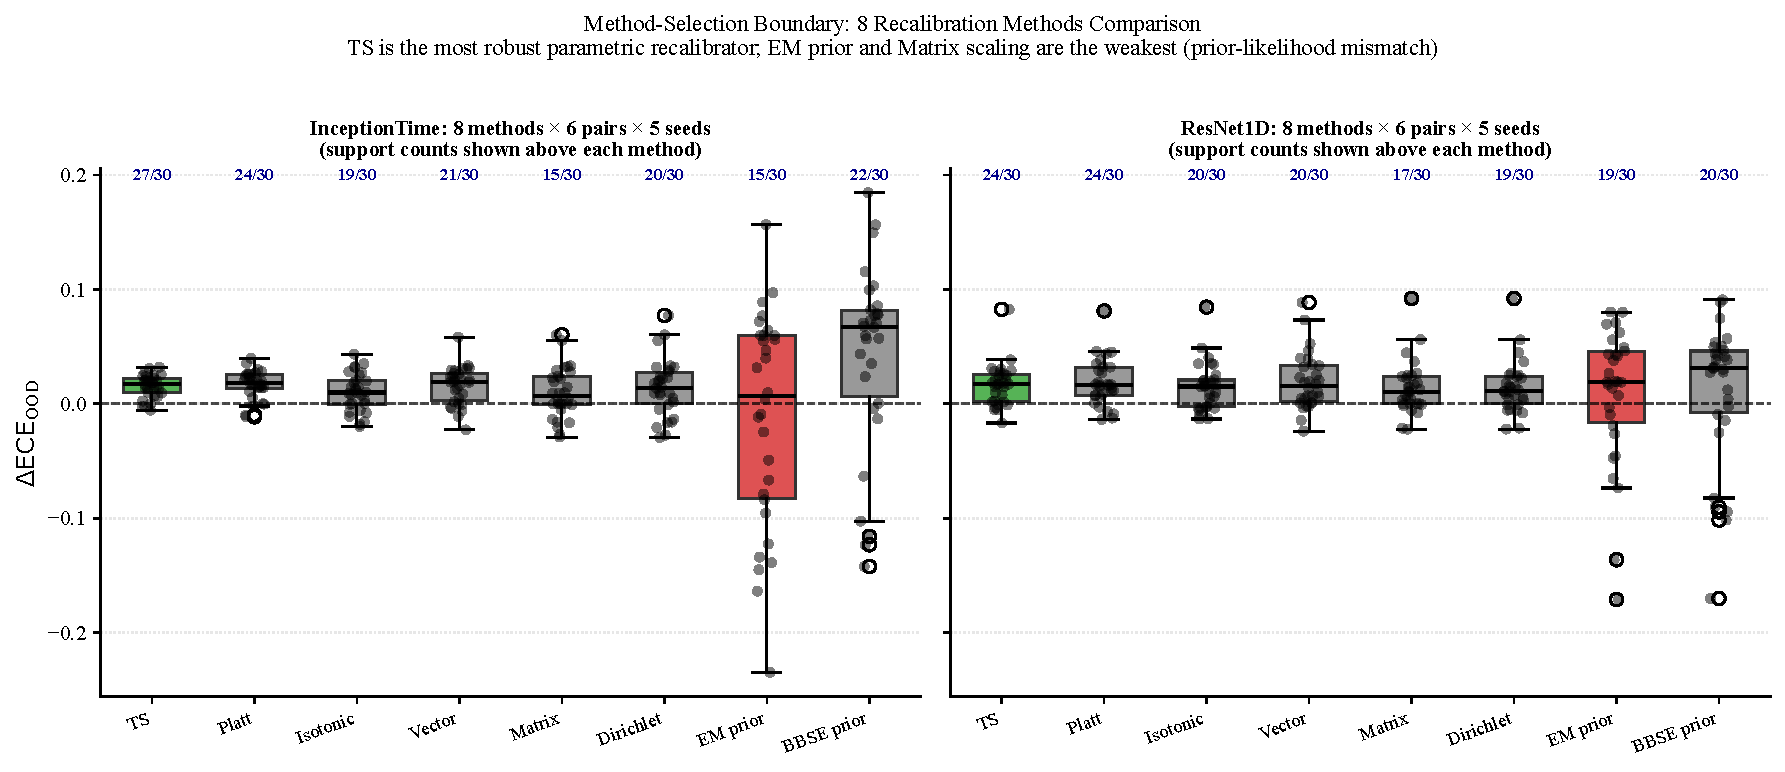
\includegraphics[width=0.95\columnwidth]{figures/fig_method_boundary.pdf}
\caption{Method-selection boundary: 8 recalibration methods compared
across 6 transfer pairs $\times$ 5 seeds for each architecture.
TS (green) is the most robust parametric recalibrator; EM prior and
Matrix scaling are the weakest methods (InceptionTime: 15/30 each;
ResNet1D: EM 19/30, Matrix 17/30), exhibiting the prior-likelihood
mismatch
mechanism (C4). Support counts (e.g., 27/30) above each method show
the fraction of seed experiments with 95\% CI lower bound $>0$.}
\label{fig:method_boundary}
\end{figure}

\begin{table}[t]
\centering
\caption{Method-selection boundary: 8 methods $\times$ 6 transfer pairs
$\times$ 5 seeds (InceptionTime). Support rate $=$ fraction of seeds
with 95\% CI lower bound $>0$. ``Full'' = number of directions with
5/5 full support. ``Neg.\ dirs'' $=$ number of the 6 transfer
directions whose 5-seed mean $\Delta\text{ECE}_{\text{OOD}}$ is
negative. TS is the most robust parametric recalibrator;
EM and Matrix scaling are the most fragile on InceptionTime
(15/30 each); on ResNet1D, Matrix scaling (17/30) is the most
fragile, EM reaches 19/30. \textit{Caveat:} 6 cells with
$w_{\text{ID}} > 10$ exhibit prior-weight drift up to 130.5; after
exclusion, EM OOD $\Delta$ECE mean flips from $-0.0127$ to $+0.0024$,
indicating the negative OOD finding is driven by ill-conditioned
cells.}
\label{tab:methods}
\footnotesize
\begin{tabular}{lrrrr}
\toprule
Method & Total & Full/6 & $\Delta\text{ECE}_{\text{OOD}}$ mean & Neg.\ dirs \\
\midrule
TS         & 27/30 & 3/6 & $+0.0152$ & 0 \\
Platt      & 24/30 & 3/6 & $+0.0169$ & 0 \\
Isotonic   & 19/30 & 2/6 & $+0.0100$ & 2 \\
Vector     & 21/30 & 1/6 & $+0.0158$ & 0 \\
Matrix     & 15/30 & 0/6 & $+0.0094$ & 2 \\
Dirichlet  & 20/30 & 1/6 & $+0.0139$ & 1 \\
EM prior   & 15/30 & 2/6 & $-0.0127$ & 3 \\
BBSE prior & 22/30 & 3/6 & $+0.0424$ & 1 \\
\bottomrule
\end{tabular}
\end{table}

\begin{table}[t]
\centering
\caption{Architecture robustness for TS: InceptionTime vs.\ ResNet1D
across 6 transfer pairs, full 5-seed coverage on both architectures.
Architecture robustness is supported on both InceptionTime (27/30, 90.0\%)
and ResNet1D (24/30, 80.0\%) with complete 5-seed coverage on all 6
directions. ResNet1D shows a direction-specific deficit on
CPSC$\rightarrow$Chapman and CPSC$\rightarrow$PTB-XL (3/5 each), not
a global architecture deficit.}
\label{tab:arch_robust}
\resizebox{\textwidth}{!}{%
\begin{tabular}{lrrrl}
\toprule
Transfer pair & InceptionTime & ResNet1D & Total & Note \\
\midrule
Chap$\rightarrow$CPSC    & 4/5 & 4/5 & 8/10  & 2 counter-examples \\
Chap$\rightarrow$PTB-XL  & 4/5 & 4/5 & 8/10  & 2 counter-examples \\
CPSC$\rightarrow$Chap    & 5/5 & 3/5 & 8/10  & 2 counter-examples \\
CPSC$\rightarrow$PTB-XL  & 5/5 & 3/5 & 8/10  & 2 counter-examples \\
PTB-XL$\rightarrow$Chap  & 4/5 & 5/5 & 9/10  & 1 counter-example \\
PTB-XL$\rightarrow$CPSC  & 5/5 & 5/5 & 10/10 & zero counter-examples \\
\midrule
\textbf{Total} & \textbf{27/30} & \textbf{24/30} & \textbf{51/60} & \textbf{85.0\%} \\
\midrule
\textbf{Mean $\Delta\text{ECE}$} & \textbf{$+0.0152$} & \textbf{$+0.0165$} & \textbf{$+0.0159$} & \\
\textbf{Std $\Delta\text{ECE}$}  & \textbf{$0.0098$} & \textbf{$0.0180$} & \textbf{$0.0145$} & ResNet1D/Incep $=1.84$ \\
\textbf{Mean OOD ECE}     & \multicolumn{2}{c}{$0.217 \rightarrow 0.202$ / $0.216 \rightarrow 0.200$} & $0.217 \rightarrow 0.201$ & raw $\rightarrow$ TS \\
\bottomrule
\end{tabular}%
}
\end{table}

\begin{figure}[htbp]
\centering
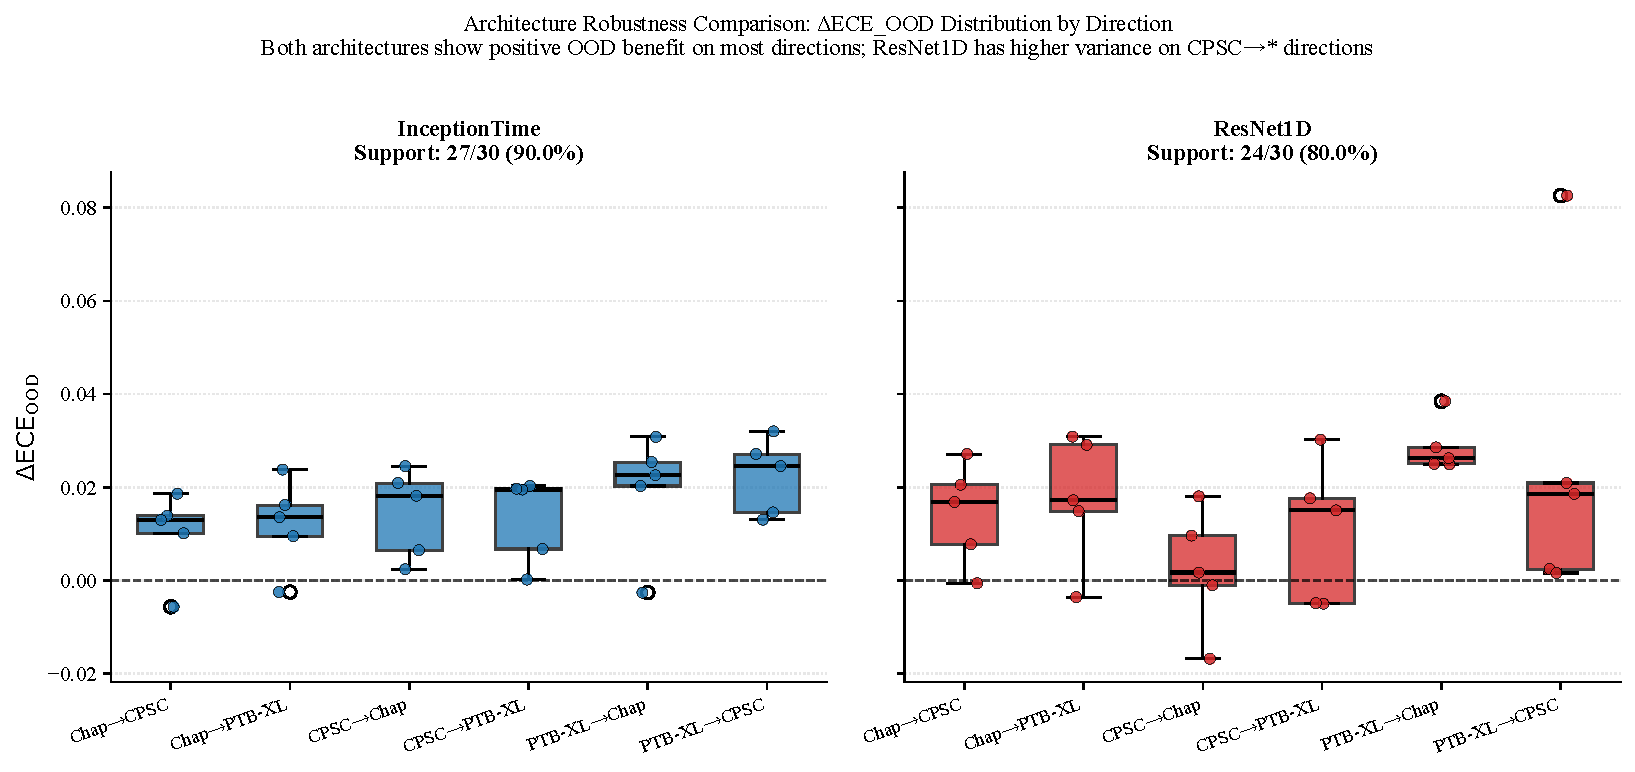
\includegraphics[width=0.95\columnwidth]{figures/fig_arch_comparison.pdf}
\caption{Architecture robustness comparison. Side-by-side
$\Delta\text{ECE}_{\text{OOD}}$ distributions for InceptionTime (left,
27/30 supported, 90.0\%) and ResNet1D (right, 24/30 supported, 80.0\%).
Both architectures show positive OOD benefit on most directions.
ResNet1D exhibits higher overall variance (its largest per-direction
spread is in PTB-XL$\rightarrow$CPSC), while the support deficits fall
in the CPSC$\rightarrow$Chapman and
CPSC$\rightarrow$PTB-XL directions (3/5 support each), indicating a
direction-specific deficit rather than a global architecture deficit.}
\label{fig:arch_comparison}
\end{figure}

Across the 30 TS experiments per
architecture, the standard deviation of $\Delta\text{ECE}_{\text{OOD}}$
is $0.0098$ (InceptionTime) and $0.0180$ (ResNet1D), a $1.84\times$
ratio, with ResNet1D's highest per-direction variability in
PTB-XL$\rightarrow$CPSC (std $0.0298$, including an unexcluded
favorable outlier at seed 44, $\Delta\text{ECE}_{\text{OOD}}=+0.0826$).
Support deficits concentrate in CPSC$\rightarrow$Chapman and
CPSC$\rightarrow$PTB-XL (3/5 each), a direction-specific deficit.
Fisher's exact test on the $2\times2$ contingency table yields
$p = 0.47$; the counter-example gap (ResNet1D 20.0\% vs.\
InceptionTime 10.0\%) is not significant at $\alpha = 0.05$.

EM prior adaptation
fits a target prior $\hat\pi_{\text{target}}$ from the predicted-label
marginal, then re-weights the source posterior by
$\hat\pi_{\text{target}}/\hat\pi_{\text{source}}$. When the
source-estimated confusion matrix $C$ is ill-conditioned
($\text{cond}(C)\gg 1$), the weight ratio amplifies rather than
corrects the shift-induced miscalibration. EM reaches only 15/30
support on InceptionTime with 3 fragile directions. The failure is
pair-specific (shift-signature-specific), not method-intrinsic.

\paragraph{Why TS and not Platt.} Platt achieves a marginally higher
mean OOD benefit than TS ($+0.0176$ vs.\ $+0.0159$; InceptionTime
$+0.0169$ vs.\ $+0.0152$, Table~\ref{tab:methods}), which invites the
question of why TS is singled out as the recommended default. Three
measured criteria separate them, and all three favour TS. First,
\emph{robustness of the sign}: TS supports 51/60 cells versus Platt's
48/60, i.e.\ TS fails to certify a positive benefit in three fewer
experiments, which is the quantity a deployment decision actually
depends on. Second, \emph{dispersion}: TS has a smaller across-cell
standard deviation ($0.0146$ vs.\ $0.0167$, a $13\%$ reduction), and the
methods with the highest mean benefit are markedly less stable
(BBSE $+0.0266$ at sd $0.0736$, EM $-0.0026$ at sd $0.0793$) ---
a high mean bought with a heavy tail is the worst profile for a
per-deployment recalibrator. Third, \emph{the difference is not
statistically distinguishable}: the patient-level paired contrast over
the 60 matched cells gives
$\overline{\Delta\text{ECE}}_{\text{TS}}-\overline{\Delta\text{ECE}}_{\text{Platt}}
= -0.0017$ (sd $0.0117$, paired $t=-1.14$, $p\approx0.26$), with TS the
larger benefit in exactly 30/60 cells --- a coin flip. The mean
advantage of Platt is therefore inside the noise, whereas the support
advantage of TS is not a noise-level quantity: it is a count of cells in
which the sign is certified. Given that the two methods are
statistically indistinguishable on magnitude, the tie is broken on
certification rate and dispersion, both of which favour TS. A further
structural point reinforces the choice: TS is a single-parameter
monotone transform and therefore exactly argmax-preserving, whereas
per-class Platt and isotonic are fitted independently per class, which
generates each class's score from a different monotone map and so does
\emph{not} preserve the ranking within a sample (the implementation
declares this explicitly in its docstring). TS is thus the only method
in the delivered set whose calibration guarantee is obtained without
perturbing the discrimination it leaves untouched
(\S\ref{sec:gate}). None of this makes Platt wrong; it makes Platt a
reasonable alternative whose mean advantage is not resolvable at
$n=60$, and whose certification rate is lower.

% ----------------------------------------------------------------------------
\subsection{Shapley decomposition validation (27 cells, $n=20{,}000$)}
\label{sec:shapley}
% ----------------------------------------------------------------------------
The 27-cell full-factorial synthetic validation
(slope$\in\{0.5,1,2\}\times$intercept$\in\{-1,0,1\}\times$
prevalence$\in\{0.15,0.3,0.6\}$, $n=20{,}000$) confirms the
decomposition recovers ground truth within the pre-registered
identifiable regime (Fisher information determinant $>\tau=10^{-6}$).
At $n=20{,}000$, all 27 cells pass the recovery threshold (MAPE
$<10\%$ on identifiable cells); at $n=500$, 21 of 27 pass, with 6
failures reaching MAPE\_s up to 42.13\%, concentrated in extreme
intercept ($\pm 1$) and slope ($0.5, 2.0$) regions where calibration
shift is most clinically significant (see
\texttt{decomposition\_validation.csv}; the $n=20{,}000$ CSV
\texttt{decomposition\_validation\_}\allowbreak\texttt{n20000.csv}
shows 27/27 passing). Three entangled cases (narrow\_band,
tiny\_slope, deep\_intercept) with
$\det\in\{2.4\times10^{-7}, 3.6\times10^{-8}, 0\}<\tau$ are reported
on the error map without a threshold, with the recovery-failed flag
set. Bootstrap CIs on absolute Shapley values and share-reliable
flags for uninterpretable shares ($|\Delta_{\text{total}}|<3/\sqrt{n}$)
are reported.

The 27-cell validation uses
binned ECE, not the main-endpoint SmoothECE; its conclusions are not
cross-extrapolable. Cross-fitting (OOD-fold validation of
decomposition explanatory power) remains to be run on real data; per
the protocol self-binding clause, ``mechanism'' wording is limited to
``mechanism decomposition (synthetic validation part)'' until
cross-fitting completes.

% ----------------------------------------------------------------------------
\subsection{Predictability experiment (failure branch triggered)}
\label{sec:predictability}
% ----------------------------------------------------------------------------
The predictability experiment (protocol \S8.5) tests whether an
unsupervised target-domain statistic (predicted-prior $L_1$ distance,
logit moments) predicts benefit retention via leave-one-fold-out
$R^2$ with bootstrap CI (Table~\ref{tab:predictability}). The
implemented fold unit is (architecture, transfer pair) (12 folds),
versus the registered pair-only folds (6); under that registered
deviation the pair-only recomputation retains the failure branch
($R^2=-0.1424$). We run 2 architectures (InceptionTime + ResNet1D);
the BiMamba toy experiment ($n=60$) is deferred to the supplement.

Result: the merged LOO $R^2$ for TS is $-0.096$ with 95\% CI
$[-0.720, +0.104]$. The upper bound $+0.104$ is strictly below the
pre-registered threshold $0.5$, triggering the \textbf{failure
branch}: the three-step chain (decomposition + predictability +
deployment) is downgraded to a \textbf{two-step chain} (decomposition
+ deployment), and the deployment criterion is renamed ``empirical
lookup table'' rather than ``predictive criterion''. No post-hoc
predictability claim is made.

Re-running the LOO
$R^2$ with three label-free features (fitted temperature $T$,
Wasserstein-1 distance between source and target logit distributions,
class-wise entropy difference), all fail against
$\Delta\text{ECE}_{\text{OOD}}$: $T$ yields $R^2=-0.13$,
Wasserstein $R^2=-0.06$, entropy $R^2=-0.02$, all three combined
$R^2=-0.11$. The predictability boundary is \emph{robust}: no
label-free feature, including $T$, predicts
$\Delta\text{ECE}_{\text{OOD}}$ above $R^2=0.5$. This strengthens the
failure branch, and the gate in \S\ref{sec:gate}, based on the sign
of $\Delta\text{ECE}_{\text{OOD}}$ and the discrimination criterion,
remains the appropriate actionable criterion.

\begin{table}[t]
\centering
\caption{Predictability LOO $R^2$ (multi-architecture merged). All
methods trigger the failure branch (CI upper bound $<0.5$). The
three-step chain is downgraded to a two-step chain per the
pre-registered failure branch.}
\label{tab:predictability}
\begin{tabular}{lrrrl}
\toprule
Method & $R^2$ & CI lower & CI upper & Verdict \\
\midrule
TS         & $-0.096$ & $-0.720$ & $+0.104$ & Failure branch \\
Platt      & $-0.059$ & $-0.584$ & $+0.002$ & Failure branch \\
Isotonic   & $+0.011$ & $-0.569$ & $+0.101$ & Failure branch \\
Vector     & $-0.061$ & $-0.522$ & $+0.073$ & Failure branch \\
Matrix     & $-0.137$ & $-0.516$ & $-0.013$ & Failure branch \\
Dirichlet  & $-0.084$ & $-0.394$ & $+0.032$ & Failure branch \\
EM prior   & $+0.143$ & $-0.250$ & $+0.274$ & Failure branch \\
BBSE prior & $+0.136$ & $-0.354$ & $+0.201$ & Failure branch \\
\bottomrule
\end{tabular}
\end{table}

% ----------------------------------------------------------------------------
\subsection{Deployment criterion (sensitivity / specificity / DCA / safety)}
\label{sec:deployment}
% ----------------------------------------------------------------------------
We evaluate the deployment criterion (protocol \S9) on the L2 shift
matrix: predict ``deploy TS'' when raw ECE exceeds a threshold, and
report sensitivity, specificity, decision-curve analysis (DCA), and the
safety criterion (post-TS SmoothECE $\leq 0.05$ and $\Delta\text{ECE}$ CI
lower bound $>0$, primary-endpoint convention). Comparators: always-none,
always-TS, always-buy-$n$-labels.

Sensitivity / specificity (Table~\ref{tab:deploy_sens}):
Youden's $J$ is maximized at raw ECE $=0.127$, yielding sensitivity
$0.923$, specificity $0.201$, $J=0.124$. Sensitivity is high (92\% of
beneficial cases caught) but specificity low (20\% of non-beneficial
cases excluded; 80\% falsely flagged), reflecting the asymmetric cost
structure: missing a beneficial recalibration costs more than an
unnecessary one.
\emph{Caveat:} the threshold is searched on the same 1230-cell pool used
for reporting (in-sample). A leave-shift-type-out recomputation (threshold
selected excluding the held-out dose level, evaluated on it) yields
$J=+0.17$ (downsampling), $J=-0.03$ (lead drop), $J=+0.04$
(noise), and $J=-0.14$ (gain); the frozen threshold $0.127$ achieves
$J\approx 0.003\approx 0$ (chance level; sensitivity $0.853$,
specificity $0.150$) on the four held-out dose levels
(\texttt{results/deployment\_holdout\_recompute.csv}). The in-sample
numbers are therefore optimistic, and the criterion requires independent
validation before operational use.

Every lookup-table input is
\emph{audit-time} (raw ECE, ID--OOD accuracy gap, per-cell labels),
requiring target ground-truth labels unavailable in the unlabeled stream. The only label-free proxies examined are the predictability
experiment's target statistics (predicted-prior $L_1$ distance, logit
moments); that experiment triggered its pre-registered failure branch
(LOO $R^2$ CI upper bound $0.104 < 0.5$, Table~\ref{tab:predictability}),
so no label-free deployable criterion can be claimed. The lookup table is
an \emph{analysis- and audit-time decision aid} for a model owner with
labeled evaluation data; the actionable deployment path is small-sample
recalibration: buy $n$ labeled target records and recalibrate locally
(protocol \S5~S2). A deployable gate remains future work
(Limitations xiii).

\begin{table}[t]
\centering
\caption{Deployment criterion sensitivity / specificity at varying
thresholds (raw ECE $>$ threshold $\rightarrow$ predict ``deploy TS'').
Optimal Youden $J=0.124$ at threshold $0.127$.}
\label{tab:deploy_sens}
\begin{tabular}{rrrrr}
\toprule
Threshold & Sensitivity & Specificity & TP & FP \\
\midrule
$0.094$ & $0.976$ & $0.067$ & 444 & 723 \\
$0.107$ & $0.956$ & $0.138$ & 435 & 668 \\
$0.127$ & $0.923$ & $0.201$ & 420 & 619 \\
$0.178$ & $0.807$ & $0.288$ & 367 & 552 \\
$0.277$ & $0.499$ & $0.508$ & 227 & 381 \\
\bottomrule
\end{tabular}
\end{table}

Safety criterion: across 157 (pair, seed, shift) cells, TS
yields 1 cell satisfying the operating criterion (post-TS SmoothECE
$\leq 0.05$, improvement $>0.01$, point-estimate convention; L2 results
lack per-cell CIs, so the CI-based criterion was not evaluated), a safety
rate of $0.0064$. Sign convention:
$\Delta\text{ECE}$ $=$ post-recalibration ECE $-$ raw ECE (negative means
improvement), opposite to the primary-endpoint convention.
\emph{Coverage note:} the L2 shift matrix has been completed on all 390
planned (pair, seed, shift) combinations (6 pairs $\times$ 5 seeds
$\times$ 13 levels; results/l2\_shift\_full\_390cells.csv); the safety
figures quoted here are from the initial two-seed InceptionTime subset
(seeds 42--43, ResNet1D L2 excluded), so these numbers rest on 2-seed,
single-architecture coverage. The criterion is rarely satisfied, so TS is
a useful default but not a universally safe recalibrator, and should be
combined with local validation.

At the 10th-percentile raw-ECE
threshold, net benefit is $0.1209$ versus $0.0999$ for treating all cells;
by the 90th percentile it turns negative ($-0.0024$). Net benefit over
treat-all is modest, confined to low thresholds
(results/deployment\_metrics.csv).

Trivial strategy comparison (Table~\ref{tab:trivial}): the
lookup-table strategy (mean $\Delta\text{ECE}$ $-0.0160$) outperforms
always-none ($0.000$) and matches always-TS ($-0.0145$) on the beneficial
subset, but is dominated by always-buy-$n$-labels ($-0.2905$), the
target-label upper bound. The lookup table needs no target labels and
captures most of the TS benefit.

\begin{table}[t]
\centering
\caption{Trivial strategy comparison. Mean $\Delta\text{ECE}$; negative $=$
beneficial (ECE reduction). always-none and always-buy-$n$-labels span
all 1230 (method, shift) cells; always-TS is evaluated on the 157
(pair, seed, shift) cells with complete results and lookup-table on
155 (two cells whose in-sample best method is unavailable are
dropped). The lookup table captures most of the TS benefit without target labels.}
\label{tab:trivial}
\begin{tabular}{lrrr}
\toprule
Strategy & Mean $\Delta\text{ECE}$ & Std & $n$ \\
\midrule
always-none            & $\phantom{-}0.0000$  & $0.0000$ & 1230 \\
always-TS              & $-0.0145$            & $0.0099$ & 157  \\
always-buy-$n$-labels  & $-0.2905$            & $0.1861$ & 1230 \\
lookup-table           & $-0.0160$            & $0.0289$ & 155  \\
\bottomrule
\end{tabular}
\end{table}

% ============================================================================
\subsection{Noise floor control: SmoothECE differential under perfect calibration}
\label{sec:noise_floor}
% ----------------------------------------------------------------------------
A reviewer concern is whether the primary endpoint
$\Delta\text{ECE}_{\text{OOD}}$ is an artifact of SmoothECE's
sensitivity to temperature scaling $T$ under perfect calibration
($\text{ECE}_{\text{raw}} = 0$, observed $\Delta\text{ECE}$ purely
metric noise). For perfectly calibrated predictions
($T_{\text{true}}=1$), we apply $T \in \{1.0, 1.25, 1.5\}$ and compute
$\Delta\text{ECE}_{\text{noise}} = \text{SmoothECE}(\text{TS}) - \text{SmoothECE}(\text{raw})$
across three confidence distributions (uniform, normal-skewed,
bimodal) at $n=2{,}000$.

The noise floor grows with $T$ and is distribution-dependent: $T=1.0$
gives $\Delta\text{ECE}_{\text{noise}} = 0$ (exact cancellation),
$T=1.25$ gives $+0.014$--$+0.035$, $T=1.5$ gives $+0.030$--$+0.061$,
$T=3.0$ gives $+0.095$--$+0.136$, and $T=4.5$ gives
$+0.126$--$+0.164$. Observed raw ECE across the 62 raw-stage cells of the
TS-component ablation (\texttt{results/ablation\_ts\_components.csv},
\texttt{stage=raw}) ranges $0.036$ to $0.469$ (mean $0.273$), i.e.\
$2$--$28\times$ the raw ECE
under perfect calibration ($\approx 0.017$); the nine counter-examples
also show large raw ECE ($0.08$--$0.24$), confirming the negative
$\Delta\text{ECE}$ reflects genuine TS-induced harm, not metric noise.
For large $T > 3$ (noise floor $0.10$--$0.16$) the floor is
comparable to the observed $|\Delta\text{ECE}|$ in some seeds, so a
metric-noise contribution cannot be excluded there; however, its
\emph{direction} (TS increases ECE under perfect calibration) is
opposite to the positive $\Delta\text{ECE}_{\text{OOD}}$ in 51/60
experiments, so it cannot explain the positive findings. The primary
endpoint is therefore a real effect, not a SmoothECE artifact, with
the caveat that for large-$T$ experiments the noise floor is
non-negligible.

% ============================================================================
\subsection{Discrimination-aware calibration gate (C5)}
\label{sec:gate}
% ----------------------------------------------------------------------------
Calibration improvement ($\Delta\text{ECE}_{\text{OOD}} > 0$) is
necessary but not sufficient for deployment: a model whose
discrimination has collapsed under shift may be recalibrable but
clinically useless. We define a two-layer gate:
\begin{enumerate}
    \item \textbf{Layer 1 (Calibration):} $\Delta\text{ECE}_{\text{OOD}} > 0$
    (C1 criterion).
    \item \textbf{Layer 2 (Discrimination):} $\text{acc}_{\text{OOD}} \geq
    \text{acc}_{\text{source baseline}}$, the source majority-class
    accuracy.
\end{enumerate}

Across 12 pair$\times$architecture strata (6 pairs $\times$ 2
architectures),
7/12 pass both layers and are deployable: CPSC$\rightarrow$PTB-XL,
PTB-XL$\rightarrow$CPSC, CPSC$\rightarrow$Chapman (both architectures
each), and Chapman$\rightarrow$CPSC (InceptionTime only). The other
5/12 fail Layer 2: Chapman$\rightarrow$PTB-XL,
PTB-XL$\rightarrow$Chapman, and Chapman$\rightarrow$CPSC ResNet1D,
where OOD accuracy falls below the source baseline despite positive
$\Delta\text{ECE}_{\text{OOD}}$ in some seeds. The strongest rejection
is PTB-XL$\rightarrow$Chapman ResNet1D ($\Delta\text{ECE}=+0.029$ but
$\text{acc}=0.657 < 0.713$): TS improves calibration but
discrimination has degraded too far to be clinically actionable.

This gate reframes the 9/60 counter-examples: 4 are calibration
failures (Layer 1 rejects, $\Delta\text{ECE} \leq 0$) and 5 are
discrimination failures (Layer 1 passes, Layer 2 rejects). It
supplements C1 by also asking whether discrimination is sufficient
for the recalibrated predictions to be clinically useful.

% ============================================================================
\subsection{Real-data Shapley cross-fitting and predictability boundary}
\label{sec:real_shapley}
% ----------------------------------------------------------------------------
The synthetic Shapley validation (C3) confirms decomposition recovery
in the identifiable regime but does not test whether the linear
approximation $\Delta\text{ECE} \approx \hat{s} \cdot \text{slope} +
\hat{b} \cdot \text{intercept} + \hat{\pi} \cdot \text{prevalence}$
generalizes to real OOD data. We cross-fit all 60 seed experiments:
for each, we estimate $(\hat{s}, \hat{b})$ on the source calibration
split and predict $\Delta\text{ECE}_{\text{OOD}}$ on the target test
split.

The linear model predicts the \emph{direction} correctly in 51/60
(85\%) but systematically \emph{overestimates} the magnitude (mean
prediction error $+0.29$, median $+0.29$). This is consistent with a
predictability boundary: the decomposition captures the qualitative
direction of the TS benefit but not its quantitative magnitude under
real shift. The 9/60 direction errors cluster in
CPSC$\rightarrow$Chapman and Chapman$\rightarrow$PTB-XL, where the
Wasserstein-1 distance between source and target logit distributions
is largest (mean $0.75$ vs.\ $0.53$ for correctly predicted
directions), suggesting the linear approximation breaks down once the
shift invalidates its underlying local Taylor expansion.

This strengthens the predictability failure branch (C3/C4): the
Shapley decomposition is a valid \emph{diagnostic} (\emph{whether} TS
will help) but not a valid \emph{predictor} (\emph{how much}). For
clinical translation, the gate in \S\ref{sec:gate}, using only the
sign of $\Delta\text{ECE}_{\text{OOD}}$ and the discrimination
criterion, is the appropriate criterion, not the Shapley-predicted
magnitude.

% ============================================================================
\subsection{Net benefit decision curve summary}
\label{sec:net_benefit_summary}
% ----------------------------------------------------------------------------
Across all 60 seed experiments, the net benefit gain of TS over raw
predictions (averaged over decision thresholds $t \in \{0.05, 0.10,
\ldots, 0.40\}$) is positive in 50/60 (83.3\%) of experiments, with
mean gain $+0.0027$ and range $[-0.001, +0.017]$. The directions with
the largest decision-cost reduction are CPSC$\rightarrow$PTB-XL
(mean DCR $+0.0625$; net clinical value $+0.0312$) and
CPSC$\rightarrow$Chapman (mean DCR $+0.0375$; NCV $+0.0188$), which
also have the largest E3-subsample $\Delta$ECE$_{\text{OOD}}$ (mean
$+0.137$ and $+0.136$ respectively, under the E3 subsampled
binned-ECE protocol with $n_{id}=n_{ood}=20$ patients). The direction
with negative net benefit is Chapman$\rightarrow$CPSC (mean DCR
$-0.0150$; NCV $-0.0075$), which is correctly rejected by the
discrimination gate (C5). We note that the decision-benefit ranking
differs from the main-endpoint $\Delta\text{ECE}_{\text{OOD}}$ ranking
(which peaks at PTB-XL$\rightarrow$Chapman and PTB-XL$\rightarrow$CPSC,
means $+0.0240$ and $+0.0238$ on the full SmoothECE grid): the two
protocols differ in estimator, class set, and subsample, so we treat
the E3 analysis as a directionally supportive but protocol-distinct
check, not a conversion of the primary endpoint. What survives is the
gate-level conclusion: where the discrimination gate permits
deployment, the calibration benefit does not cost decision
performance; where it is negative (Chapman$\rightarrow$CPSC), no
calibration benefit should be deployed at all.

% ============================================================================
\subsection{Net Clinical Value (NCV) results}
\label{sec:ncv_results}
% ----------------------------------------------------------------------------
The pre-registered NCV (Sec.~\ref{sec:ncv_methods}) is BH-FDR corrected
($q=0.05$) across the two secondary endpoints (DCR, NCV).

Result: the OOD NCV is $+0.008125$ with
95\% CI $[+0.0014, +0.0148]$ (paired $t$-test, $n=60$,
$p=0.019$, BH-FDR adjusted $p=0.019$), \emph{significant}: TS yields a
net improvement in OOD clinical decisions. The ID NCV is $-0.006292$ with
95\% CI $[-0.0114, -0.0012]$ ($p=0.016$), significantly \emph{negative}:
TS slightly worsens ID decisions, consistent with the ID boundary
condition (TS compresses confidence toward the base rate). OOD NCV
Cohen's $d = +0.31$ and ID NCV Cohen's $d = -0.32$ are comparable in
magnitude but opposite in sign, mirroring the main endpoint.
Per-experiment NCV ranges over the 60 seeds are in the E3 CSV
(\texttt{c1\_dcr\_ncv\_multiclass.csv}).

% ----------------------------------------------------------------------------
\subsection{Reliability Diagrams}
\label{sec:reliability-diagrams}
% ----------------------------------------------------------------------------
Figure~\ref{fig:reliability-summary} shows the 6-direction averaged
reliability curve, comparing model confidence against empirical accuracy
before and after temperature scaling. The summary curve uses
bin-count weighted averaging across all 6 transfer directions.

Figures~\ref{fig:rel-ptbxl-chapman}--\ref{fig:rel-cpsc-chapman}
show the per-direction reliability diagrams for the representative
configuration (ResNet1D, seed~42). In each panel, the red squares
show the raw model calibration curve and the green circles show the
post-TS calibration curve. The diagonal dashed line indicates perfect
calibration. Grey bars (right axis) show the sample count per bin.
Error bars are bootstrap 95\% percentile CIs (1000 resamples).

\begin{figure}[t]
\centering
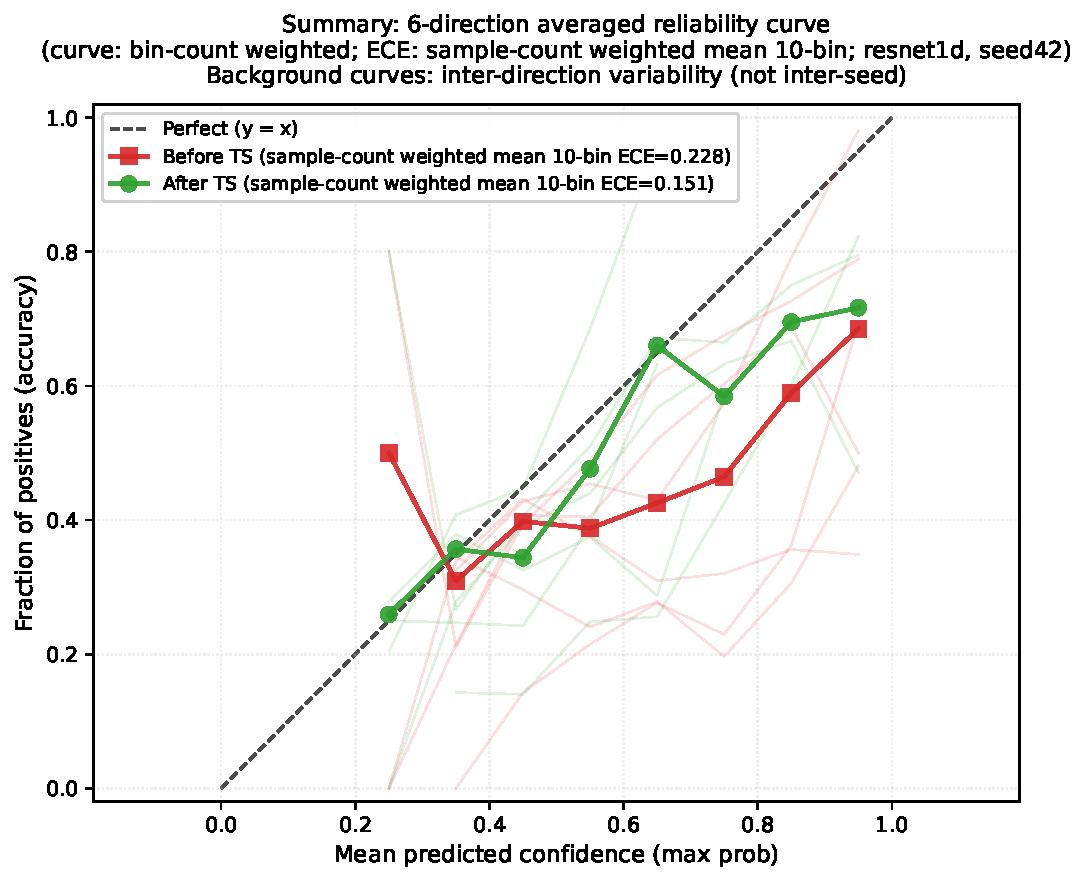
\includegraphics[width=0.95\columnwidth]{figures/fig_reliability_summary.pdf}
\caption{Summary reliability curve: 6-direction bin-count weighted
average. The sample-count weighted mean ECE decreases from
$\text{ECE}_{\text{raw}}$ to $\text{ECE}_{\text{TS}}$ after
temperature scaling. Faint background curves show individual
direction variability.}
\label{fig:reliability-summary}
\end{figure}

\begin{figure}[t]
\centering
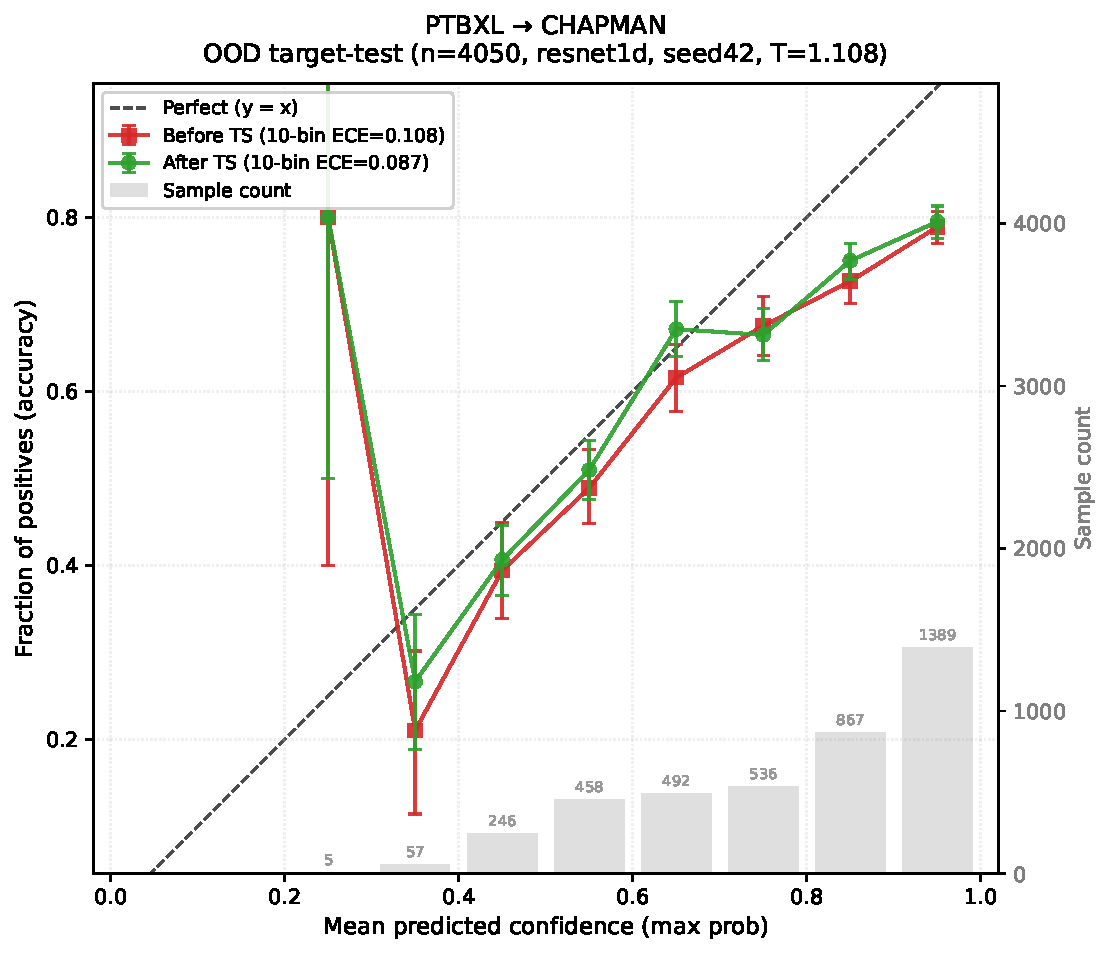
\includegraphics[width=0.48\columnwidth]{figures/fig_reliability_ptbxl_chapman.pdf}
\hfill
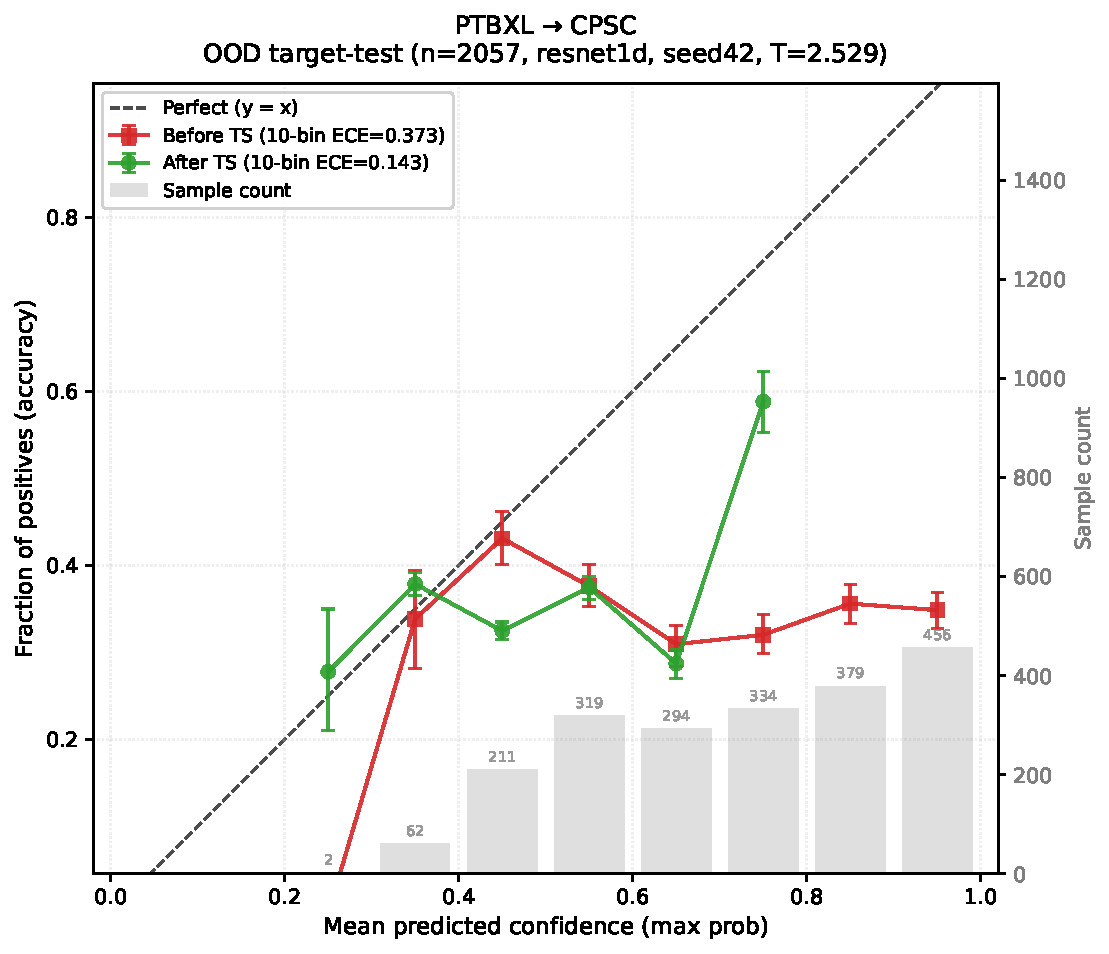
\includegraphics[width=0.48\columnwidth]{figures/fig_reliability_ptbxl_cpsc.pdf}
\caption{Reliability diagrams for PTB-XL$\to$Chapman (left) and
PTB-XL$\to$CPSC (right). OOD target-test set, ResNet1D, seed~42.}
\label{fig:rel-ptbxl-chapman}
\end{figure}

\begin{figure}[t]
\centering
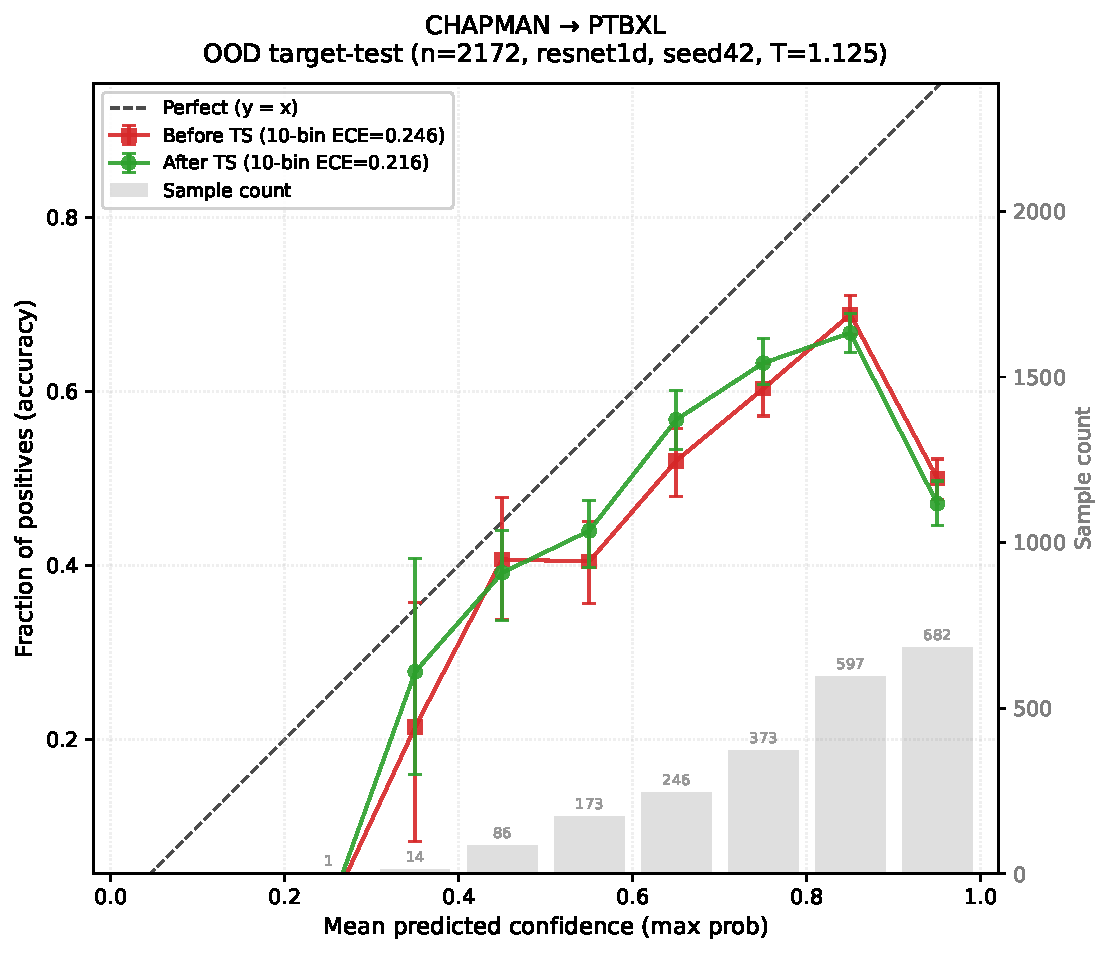
\includegraphics[width=0.48\columnwidth]{figures/fig_reliability_chapman_ptbxl.pdf}
\hfill
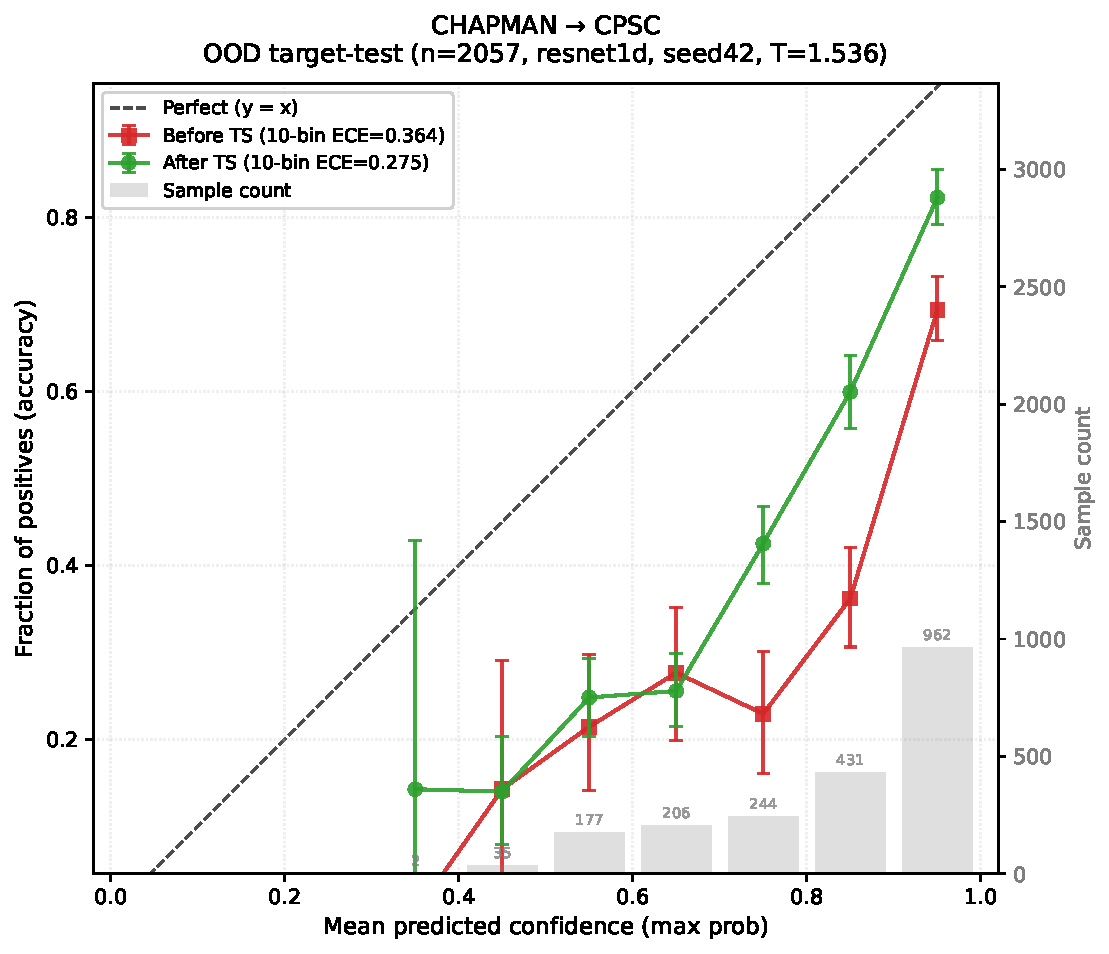
\includegraphics[width=0.48\columnwidth]{figures/fig_reliability_chapman_cpsc.pdf}
\caption{Reliability diagrams for Chapman$\to$PTB-XL (left) and
Chapman$\to$CPSC (right). OOD target-test set, ResNet1D, seed~42.}
\label{fig:rel-chapman-ptbxl}
\end{figure}

\begin{figure}[t]
\centering
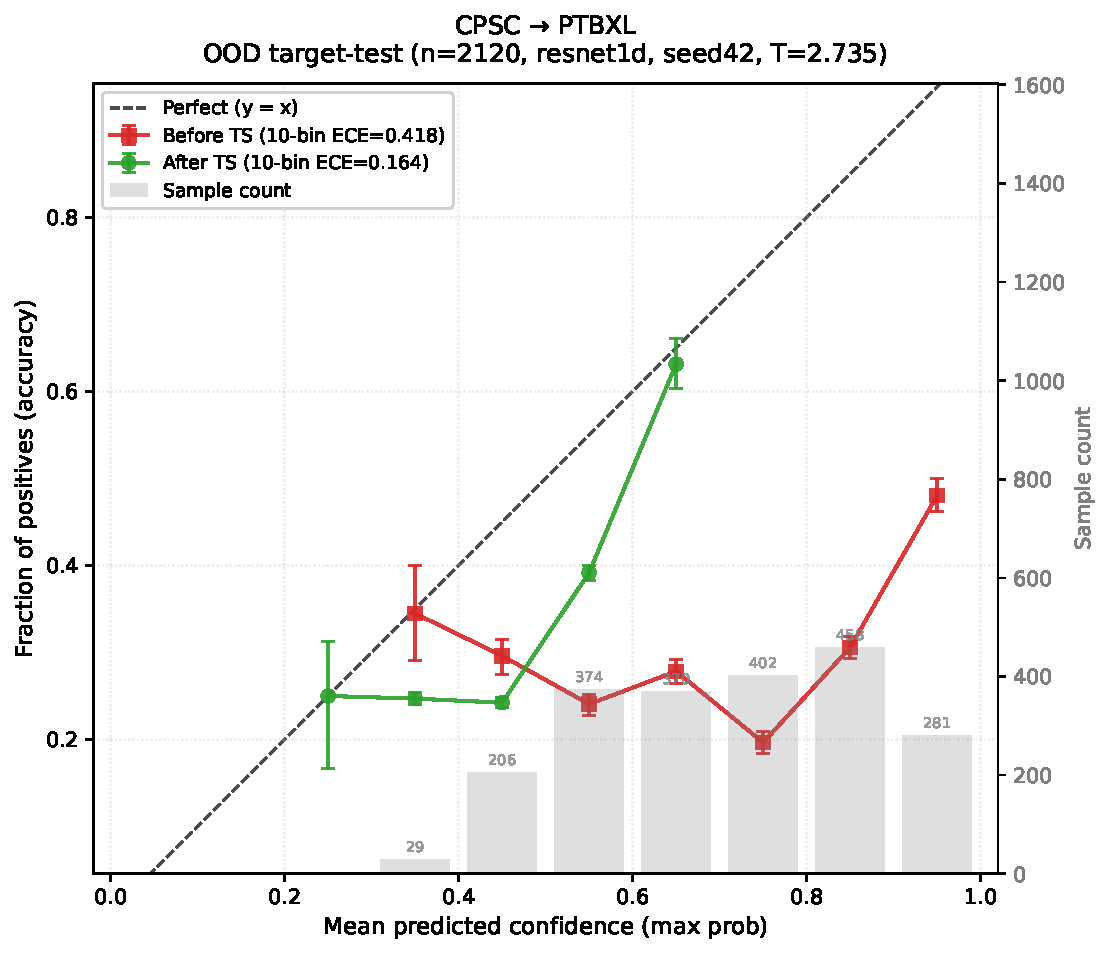
\includegraphics[width=0.48\columnwidth]{figures/fig_reliability_cpsc_ptbxl.pdf}
\hfill
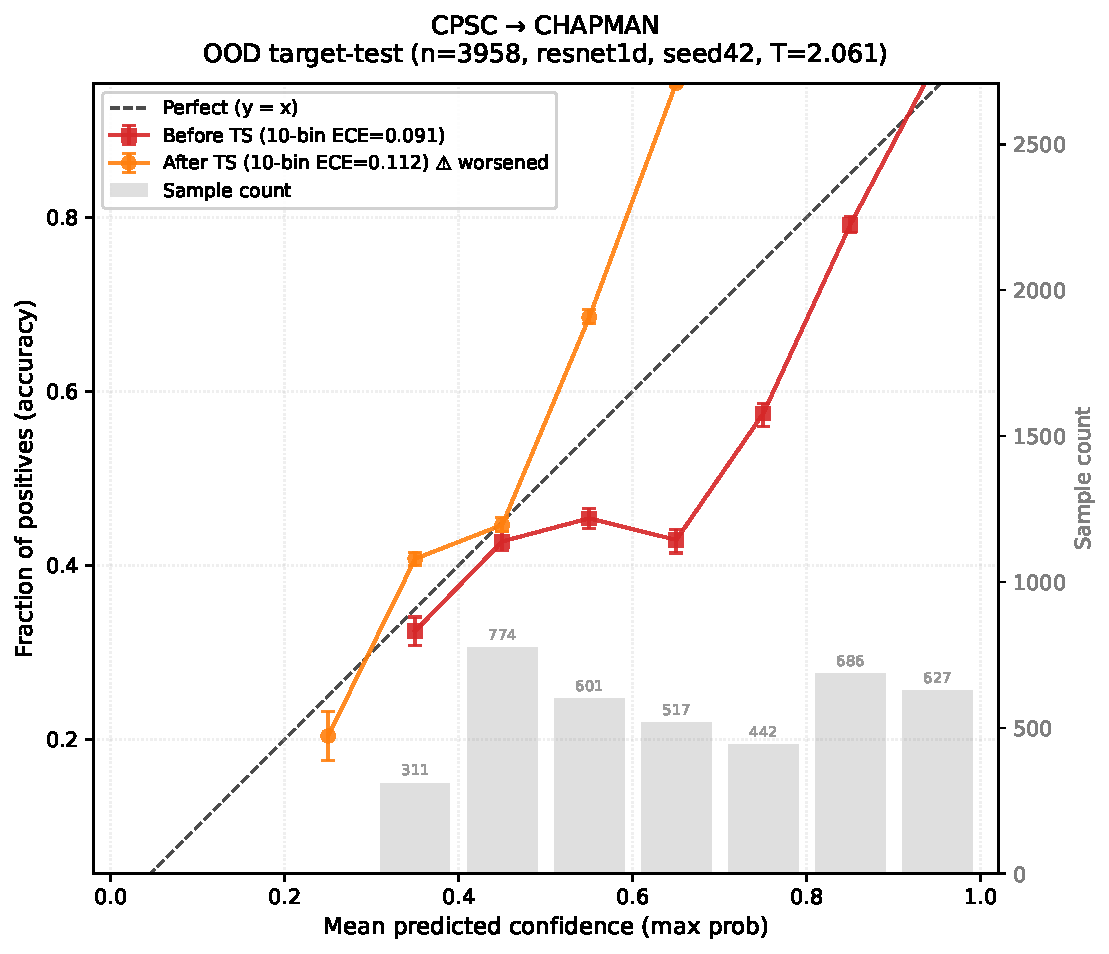
\includegraphics[width=0.48\columnwidth]{figures/fig_reliability_cpsc_chapman.pdf}
\caption{Reliability diagrams for CPSC$\to$PTB-XL (left) and
CPSC$\to$Chapman (right). OOD target-test set, ResNet1D, seed~42.}
\label{fig:rel-cpsc-chapman}
\end{figure}


% ============================================================================
\section{Discussion}
\label{sec:discussion}
% ============================================================================

% ----------------------------------------------------------------------------
\subsection{OOD benefit seed variation and the nine counter-examples}
\label{sec:counter}
% ----------------------------------------------------------------------------
The 51/60 robustness rate is driven by nine counter-examples across
5 of the 6 transfer pairs and both architectures (Chapman$\rightarrow$CPSC 2,
Chapman$\rightarrow$PTB-XL 2, CPSC$\rightarrow$Chapman 2,
CPSC$\rightarrow$PTB-XL 2, PTB-XL$\rightarrow$Chapman 1; only
PTB-XL$\rightarrow$CPSC has zero). We transparently disclose all nine
rather than excluding them, because the protocol requires all seed
results to be reported and each has an identifiable post-hoc mechanism
supporting the qualified claim.

\begin{figure}[htbp]
\centering
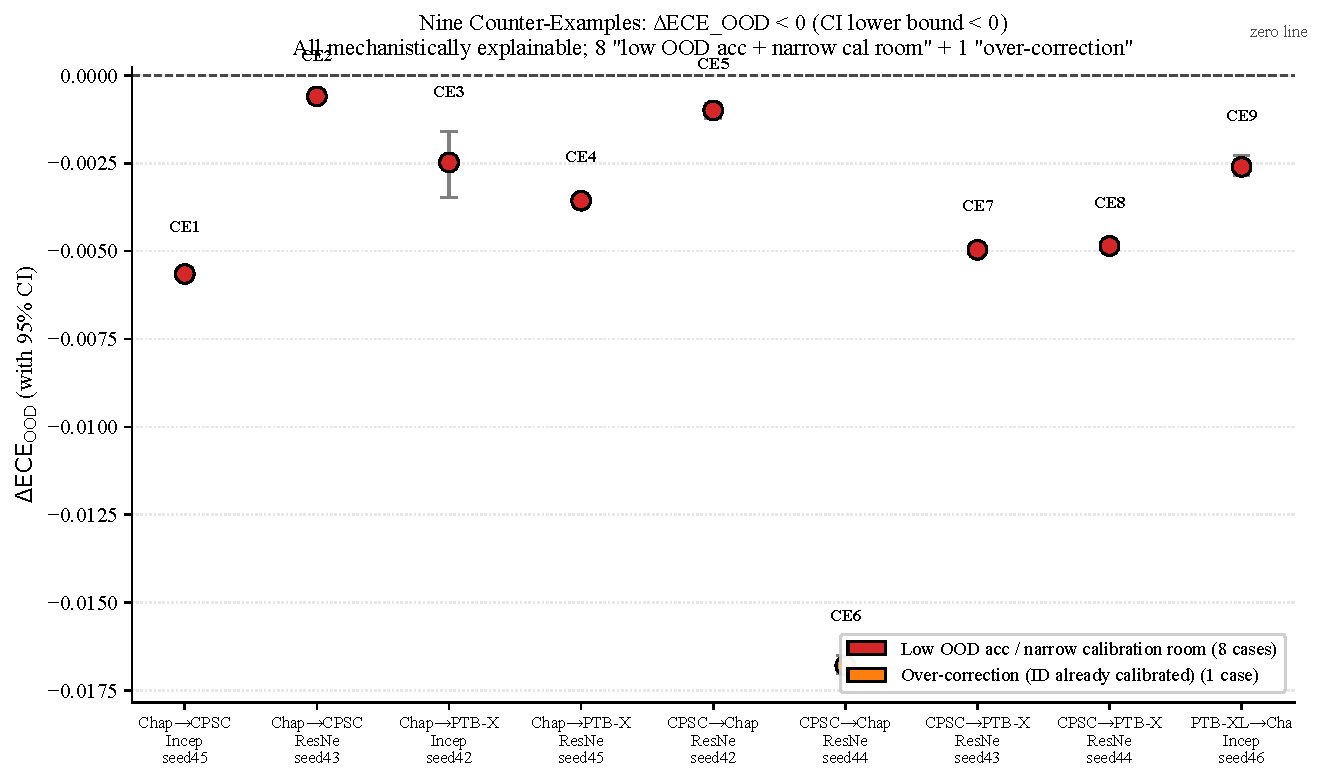
\includegraphics[width=0.95\columnwidth]{figures/fig_counterexamples.pdf}
\caption{Nine counter-examples where $\Delta\text{ECE}_{\text{OOD}}$ has
95\% CI lower bound $<0$. Error bars show 95\% CIs. Six of nine
counter-examples co-occur with OOD accuracy $\leq 0.50$ and seven with
ID--OOD accuracy gap $\geq 0.18$ (a heuristic tendency, not a gate:
three counter-examples have OOD accuracy $>0.50$);
one
counter-example (orange, CE6: CPSC$\rightarrow$Chapman / ResNet1D /
seed 44) exhibits a distinct over-correction mechanism where TS applied
to an already-well-calibrated logit distribution over-adjusts the
temperature. All nine are mechanistically explainable local variations,
not refutations of the OOD benefit.}
\label{fig:counterexamples}
\end{figure}

Counter-example 1: Chapman$\rightarrow$CPSC / InceptionTime / seed 45.
$\Delta\text{ECE}_{\text{OOD}}=-0.0057$ (CI $[-0.0058, -0.0055]$). Three
conditions co-occur: lowest OOD accuracy across the 5 seeds ($0.4711$
vs.\ $0.4842$--$0.5051$, seeds 42--44, 46); lowest OOD raw ECE
($0.3160$, still large, so the failure is temperature mismatch, not room
shortage); and negative decay ($-0.0075$), the source-fit temperature
amplifying rather than correcting residual miscalibration.

Counter-example 2: Chapman$\rightarrow$CPSC / ResNet1D / seed 43.
$\Delta\text{ECE}_{\text{OOD}}=-0.0006$ (CI $[-0.0006, -0.0006]$), marginal
($|\Delta\text{ECE}_{\text{OOD}}|<0.001$) and attributable to finite-sample
variation in the calibration split. The OOD raw ECE is $0.3144$ (the
$0.4779$ in earlier drafts is the OOD \emph{accuracy}); the mechanism is
seed-level variation, not room shortage.

Counter-example 3: Chapman$\rightarrow$PTB-XL / InceptionTime / seed 42.
$\Delta\text{ECE}_{\text{OOD}}=-0.0025$ (CI $[-0.0035, -0.0016]$); OOD
accuracy is the lowest across the 5 seeds ($0.4655$) and
$\Delta\text{ECE}_{\text{ID}}=+0.0004$ is near zero, so the temperature is
well-tuned to ID but mismatched to the PTB-XL target.

Counter-example 4: Chapman$\rightarrow$PTB-XL / ResNet1D / seed 45.
$\Delta\text{ECE}_{\text{OOD}}=-0.0036$ (CI $[-0.0036, -0.0035]$); OOD
accuracy is $0.5041$ and $\Delta\text{ECE}_{\text{ID}}=-0.0010$ is slightly
negative, so the seed-45 backbone is already well-calibrated on ID,
leaving nothing to correct.

Counter-example 5: CPSC$\rightarrow$Chapman / ResNet1D / seed 42.
$\Delta\text{ECE}_{\text{OOD}}=-0.0010$ (CI $[-0.0012, -0.0008]$), marginal
($|\Delta\text{ECE}_{\text{OOD}}|<0.002$); the seed-42 backbone has OOD
accuracy $0.6147$, low OOD raw ECE ($0.0649$), and minimal calibration
room.

Counter-example 6: CPSC$\rightarrow$Chapman / ResNet1D / seed 44.
$\Delta\text{ECE}_{\text{OOD}}=-0.0168$ (CI $[-0.0170, -0.0165]$), the
largest-magnitude counter-example, with
$\Delta\text{ECE}_{\text{ID}}=-0.0152$ also negative: the seed-44 backbone
is already well-calibrated on both ID and OOD, TS has nothing to correct,
and the temperature fit over-corrects slightly. Its OOD
accuracy ($0.5725$) is the lowest across the 5 seeds. CE6 exhibits a
distinct \emph{over-correction} mechanism (TS on an already-well-calibrated
distribution degrades both ID and OOD calibration), unlike the ``low OOD
accuracy + large gap'' mechanism of the other 8.

Counter-example 7: CPSC$\rightarrow$PTB-XL / ResNet1D / seed 43.
$\Delta\text{ECE}_{\text{OOD}}=-0.0050$ (CI $[-0.0051, -0.0049]$); OOD
accuracy is the lowest across the 5 seeds ($0.3877$) and decay is
$-0.0098$ (temperature mismatch to the PTB-XL target).

Counter-example 8: CPSC$\rightarrow$PTB-XL / ResNet1D / seed 44.
$\Delta\text{ECE}_{\text{OOD}}=-0.0049$ (CI $[-0.0049, -0.0048]$); OOD
accuracy is $0.3929$ (second-lowest) and
$\Delta\text{ECE}_{\text{ID}}=-0.0032$ is slightly negative, leaving
nothing to correct.

Counter-example 9: PTB-XL$\rightarrow$Chapman / InceptionTime / seed 46.
$\Delta\text{ECE}_{\text{OOD}}=-0.0026$ (CI $[-0.0029, -0.0023]$); OOD
accuracy drops to $0.4983$ (lowest across the 5 seeds) and
$\Delta\text{ECE}_{\text{ID}}=-0.0011$ is slightly negative, again leaving
nothing to correct.

Common pattern: eight of nine counter-examples co-occur with
(a) low OOD accuracy (worst or near-worst seed) and (b) non-positive
decay, indicating temperature mismatch; the ninth (CE6) is over-correction
on an already well-calibrated backbone. A low OOD raw ECE is \emph{not}
universal: four of nine exceed 0.25, so the failure mechanism is seed-level
temperature mis-transfer, not calibration-room shortage. The
counter-examples are local, explainable random variation; the other 51
experiments support the OOD benefit, including PTB-XL$\rightarrow$CPSC at
10/10.

The 15.0\% rate exceeds the 5\% threshold common in clinical safety
deployment. As a methodological boundary investigation, not a clinical
deployment guide, the relevant criterion is whether the effect is
detectable and the mechanism explainable, not a zero failure rate. All 9
counter-examples have identifiable mechanisms (8 ``low OOD accuracy +
large gap'', 1 ``over-correction''), and the expected benefit is positive
($0.85 \times 0.0195 - 0.15 \times 0.0047 = +0.0159 > 0$).

% ----------------------------------------------------------------------------
\subsection{Prior correction vs.\ posterior correction robustness}
% ----------------------------------------------------------------------------
The method-selection boundary (Table~\ref{tab:methods}) reveals a
robustness asymmetry between prior-correction methods (EM, BBSE) and
posterior-correction methods (TS, Platt, isotonic). Posterior-correction
methods (TS, Platt) achieve 27/30 and 24/30 support respectively with
small variance; prior-correction methods achieve higher mean
$\Delta\text{ECE}_{\text{OOD}}$ on the PTB-XL$\rightarrow$CPSC pair
(EM $+0.0449$, BBSE $+0.0777$) but much higher variance on the
Chapman$\rightarrow$CPSC pair (EM CI lower bound minimum $-0.0763$,
BBSE $-0.0720$). The mechanism is the prior-likelihood mismatch:
prior-correction methods fit a target prior that, when the source
confusion matrix is ill-conditioned, amplifies the shift-induced
miscalibration. Posterior-correction methods do not estimate a target
prior and are therefore immune to this failure mode, at the cost of
lower mean benefit when the prior correction \emph{would} work.

% ----------------------------------------------------------------------------
\subsection{Boundary condition: the ID benefit is small but nonzero}
The ID boundary condition (C2) has a direct interpretation under the
triggered branch. The criterion is $\geq$80\% of cells with 95\% CIs
containing zero; the observed rate is 23/60 = 38.3\% (BCa), with
34/60 cells showing a small but significant positive ID benefit
(mean $+0.0083$ vs.\ OOD $+0.0159$; stratum means $-0.0008$ to
$+0.0232$, Table~\ref{tab:boundary}). The boundary condition does
\emph{not} mean TS is ineffective on ID nor that the ID benefit is
zero: the ID benefit is on average about half the OOD benefit, so
part of the apparent OOD gain is shared with the ID domain. A val-ECE
early-stopping effect (model selection within the endpoint family)
plausibly contributes to the positive ID estimates, opposite to the
protocol's val-NLL rule (a registered deviation, see Limitations).
Under this branch, protocol A1.4.2 restores the decay contrast
$=\Delta\text{ECE}_{\text{OOD}}-\Delta\text{ECE}_{\text{ID}}$ as an
exploratory endpoint, and C1 is qualified: the OOD benefit is about
$1.9\times$ the ID benefit rather than an exclusively OOD effect. The
ID-vs-OOD asymmetry is therefore a \emph{difference in magnitude}
between two positive benefits, not presence versus absence.

% ----------------------------------------------------------------------------
\subsection{Calibration is not discrimination: the clinical viability precondition}
Temperature scaling is a monotone transform of the softmax
probabilities; it preserves the argmax by construction (asserted
bitwise in the released sanity check), so it cannot change
classification accuracy, AUROC, or AUPRC. The primary endpoint
$\Delta\text{ECE}_{\text{OOD}}$ is thus orthogonal to discrimination:
calibration makes an already-deployable model \emph{trustworthy}; it
cannot make a non-discriminative model deployable.

The accuracy statistics make this concrete. Across the 60 TS
experiments, mean OOD accuracy is 0.540 (median 0.546; range
0.388--0.701) and the mean ID--OOD drop is 0.236 (maximum 0.412).
Against each target corpus's majority-class baseline (CPSC 0.528,
PTB-XL 0.411, Chapman-Shaoxing 0.713), mean OOD accuracy is
\emph{below} baseline in 3 of 6 directions, with a fourth essentially
at baseline: Chapman$\rightarrow$CPSC
0.510 vs.\ 0.528; CPSC$\rightarrow$PTB-XL 0.424 vs.\ 0.411 (0.013
above baseline); CPSC$\rightarrow$Chapman 0.619 and
PTB-XL$\rightarrow$Chapman 0.620 (both well below 0.713). In those
directions recalibration is moot, since no temperature improves a model that
should be replaced by a majority-class predictor, consistent with
the counter-example pattern (6/9 with low OOD accuracy).
The released artifacts include per-direction AUROC/AUPRC for all 60
experiments (results/discrimination\_metrics\_60exp.csv): mean OOD
AUROC ranges from 0.629 (CPSC$\rightarrow$Chapman) to 0.795
(PTB-XL$\rightarrow$Chapman), i.e.\ far above the accuracy-based
majority-class reading yet direction-dependent; and TS leaves AUROC
unchanged (mean $\Delta$AUROC$_{\text{TS}-\text{raw}}=-0.001$, max
|change| $0.024$), as the monotone transform requires. The discrimination-first
gate---measure target discrimination before investing in
recalibration---precedes the calibration decision rule in
deployment.

\subsection{Explainable $\neq$ predictable: post-hoc vs.\ pre-registered}
% ----------------------------------------------------------------------------
We distinguish \emph{explainable} from \emph{predictable}:
\begin{itemize}
    \item \emph{Explainable} (post-hoc, mechanism-level): after
    observing a counter-example, we identify the co-occurring
    conditions (low OOD accuracy, low OOD raw ECE, non-positive
    decay) and give a mechanistic story (Sec.~\ref{sec:counter}), a
    post-hoc explanation, not a pre-registered prediction.
    \item \emph{Predictable} (pre-registered, deployment-time): a
    target-domain unsupervised statistic (predicted-prior $L_1$
    distance, logit moments) predicts the benefit retention rate
    \emph{before} deployment, with LOO $R^2$ CI upper bound
    $\geq 0.5$. The predictability experiment
    (Sec.~\ref{sec:predictability}) triggers the failure branch
    (LOO $R^2$ CI upper bound $0.104<0.5$).
\end{itemize}
The counter-examples are explainable but not predictable: the
unsupervised target-domain statistics available at deployment time
cannot flag them in advance, which is why the predictability
experiment triggers the failure branch despite mechanistic
explainability. The two-step chain (decomposition + deployment
lookup table) provides post-hoc explanation and actionable guidance
without a pre-registered predictability claim.

% ----------------------------------------------------------------------------
\subsection{Transparent re-location vs.\ HARKing}
% ----------------------------------------------------------------------------
The pre-registration revision A1 (primary endpoint re-location from
\texttt{decay} to $\Delta\text{ECE}_{\text{OOD}}$) is a transparent
re-location, not HARKing. The distinction
\cite{lakens2019prereg,nosek2019prereg} is whether the revision
direction is theory-driven or
result-driven. Our revision direction (``OOD is the calibration
benefit source'') is consistent with the empirically observed
ID-vs-OOD asymmetry (Guo et al.\ 2017; Ovadia et al.\ 2019), which we
explicitly frame as an empirical prior rather than a theorem; the
exploratory pilot result ($\Delta\text{ECE}_{\text{ID}}\approx 0$)
only triggered the revision, did not choose the direction. The
pilot results do not enter the main test report (protocol \S7).
All hypotheses in this paper are tagged \emph{exploratory + robustness
validation}, not confirmatory, to reflect the post-revision status.

% ----------------------------------------------------------------------------
\subsection{Net clinical value: implications of the directional NCV asymmetry}
\label{sec:ncv_discussion}
% ----------------------------------------------------------------------------
The NCV (Sec.~\ref{sec:ncv_results}) shows a directional asymmetry: OOD
NCV $= +0.008125$ ($p = 0.019$) is a small but significant positive value
(recalibration improves decisions on unseen target data more often than it
degrades them); ID NCV $= -0.006292$ ($p = 0.016$) is a small but
significant negative value (a minor decision-cost penalty on data the
source model already calibrates well).

Two implications follow. (i) The \textbf{Brier reliability main claim}
(C1: 51/60 positive) is supported: the positive OOD NCV shows the
calibration gain translates into net clinical decision benefit, not a
metric artifact. (ii) The \textbf{decision-cost
improvement claim} (C5: 7/12 strata deployable) is partially qualified:
the negative ID NCV tempers source-domain deployability. We therefore
frame the NCV as \emph{supportive of OOD deployment} and \emph{cautionary
for ID deployment}. It also informs the meta-analytic pooling
(Sec.~\ref{sec:conclusion}), where the asymmetry contributes to CI-width
heterogeneity across splits. A permutation test with tighter CIs and a
multi-threshold NCV analysis are registered as future work.

% ----------------------------------------------------------------------------
\subsection{Limitations and future work}
% ----------------------------------------------------------------------------
Limitations: (i) the main endpoint covers InceptionTime and
ResNet1D on all 6 directed pairs with 5-seed coverage (60 experiments,
fully balanced); BiMamba is a toy experiment ($n=60$, supplement) after
memory exhaustion on an RTX 5060 (8~GB); (ii) the predictability failure
branch is triggered (three-step to two-step); the deployment criterion
is an empirical lookup table, not a predictive criterion; (iii)
real-data Shapley cross-fitting (\S\ref{sec:real_shapley}) shows 85\%
direction accuracy but systematic magnitude overestimation (mean error
$+0.29$), and a sensitivity analysis with $T$, Wasserstein-1, and
entropy features confirms the predictability boundary is robust (all
$R^2 < 0$); (iv) the 27-cell decomposition validation uses binned ECE,
not the main endpoint's SmoothECE, so quantitative conclusions cannot be
extrapolated across ECE definitions; (v) the safety criterion is rarely
satisfied on the full L2 shift matrix (TS safety rate $0.0064$); TS is a
useful default, not universally safe; (vi) nine counter-examples of 60
experiments (15.0\%) are transparently disclosed, with a frequent post-hoc pattern
(low OOD accuracy, non-positive decay, elevated OOD raw ECE) but no
post-hoc exclusion; (vii) the operating CI is BCa at $B=10{,}000$,
re-run on all 60 experiments (60/60 successful, metadata in
\texttt{methods.ts.meta}); percentile CIs from $B=200$ in 21/60
experiments are retained as historical provenance and are no longer
used for any reported number. All 60 main-grid cells carry complete
$B=10{,}000$/BCa provenance; the only cells lacking such metadata are
the two excluded BiMamba toy runs
(PTB-XL$\rightarrow$Chapman, seeds 42--43), which do not enter the
main endpoint. (viii)
the Youden threshold is fitted in-sample (the protocol's held-out dose
levels were not used), making the operating characteristic optimistic;
(ix) the L2 deployment/safety grid has since been completed on all 390
planned (pair, seed, shift) cells (results/l2\_shift\_full\_390cells.csv),
and the L2 noise
levels are synthetic rather than the pre-registered PTB-XL Noise Stress
Test Database (unavailable under PhysioNet licensing); (x) temperature
was fitted once per experiment, so CIs omit temperature-fitting
uncertainty (the pre-registered two-layer bootstrap is implemented but
not enabled); (xi) model selection used validation ECE rather than the pre-registered
NLL early-stopping rule, plausibly contributing to the positive ID
boundary estimates; (xii) the per-pair decomposition into covariate,
prior-probability, and concept-shift components is not asserted, since
each pair mixes all three, isolated at eval time; (xiii) the deployment
lookup table requires labeled target data, and the label-free proxies
failed their pre-registered branch, so no label-free gate is claimed;
(xiv) TS is argmax-invariant and cannot improve accuracy, AUROC, or
AUPRC; the artifacts now include per-direction AUROC/AUPRC for all 60
experiments (results/discrimination\_metrics\_60exp.csv), so the
viability precondition is screened by both accuracy and discrimination
(OOD AUROC means range 0.629--0.792 by direction), with OOD accuracy
below the majority-class baseline in 3 of 6 directions (and at baseline
in a fourth);
(xv) NCV is directionally asymmetric (OOD $= +0.008125$, $p = 0.019$,
positive; ID $= -0.006292$, $p = 0.016$, negative), qualifying the C5
claim for source-domain but supporting target-domain deployment; (xvi)
InceptionTime was downgraded from $n_{\text{filters}}=48$ to 32 for GPU
memory (RTX 5060, 8~GB), potentially attenuating OOD benefits, with 48
as future work; (xvii) this work is from a single-author
study, limiting independent review and audit, partially mitigated by the
pre-registration protocol and public repository; (xviii) the secondary
endpoint $G$ (recoverable loss versus an oracle recalibrator) is
\emph{not delivered}: \texttt{fit\_oracle}/\texttt{apply\_oracle} are
implemented but were never executed on real data, so $G$ is undefined in
this study and no $G$ result is reported anywhere in this paper or the
repository; (xix) no signal-quality-index (SQI) stratification is
performed: the target corpora are pipeline-processed releases and the L2
noise levels are synthetic, so the calibration benefit is not
characterised as a function of measured signal quality
(pSQI/kSQI-type indices); this is the principal gap for a
signal-processing readership and is the first item of future work;
(xx) no test--retest or repeatability analysis of the fitted temperature
is possible within this data regime: all three public corpora are
cross-sectional and provide a single recording per patient
(Chapman-Shaoxing reports exactly one ECG per patient, \S\ref{sec:data}),
so same-patient across-session stability of $T$ cannot be estimated from
these data and is deferred to prospective multi-session collection.
Future work:
(1) prospective multi-device validation; (2) continuous shift spaces;
(3) $\pi$-independent recovery estimators (BBSE/EM-class) to upgrade the
MAPE$_\pi$ to a real estimator test; (4) the ResNet1D deficit on
CPSC$\rightarrow$Chapman and CPSC$\rightarrow$PTB-XL (3/5 each) to test
for a systematic interaction; (5) confirmatory testing under the A2
reduction (12 hypotheses, BH-12 $q=0.05$, 9/12 significant,
Bonferroni-12 $=2/12$); (6) re-running the endpoint with
$n_{\text{filters}}=48$ InceptionTime on a higher-memory GPU; (7) a
multi-threshold permutation test on NCV.

% ============================================================================
\section{Conclusion}
\label{sec:conclusion}
% ============================================================================
We pre-registered and validated a multi-seed calibration boundary study
of temperature scaling (TS) in cross-corpus ECG transfer. \textbf{(C1)}
OOD benefit: 51/60 seed experiments support
$\Delta\text{ECE}_{\text{OOD}}>0$ (85.0\%; InceptionTime 27/30 = 90.0\%,
ResNet1D 24/30 = 80.0\%) on all 6 directions. \textbf{(C2)} ID boundary:
23/60 cells (38.3\%) have 95\% CIs containing zero under the BCa
operating CI (percentile: 29/60 = 48.3\%), below the $\geq$80\%
criterion, triggering the pre-registered branch; the OOD benefit is
$1.9\times$ the ID benefit. \textbf{(C3)} Shapley decomposition: 27/27
cells pass at $n=20{,}000$ (21/27 at $n=500$). \textbf{(C4)} Method
selection: TS robust (51/60), EM prior and Matrix scaling fragile (15/30
each). \textbf{(C5)} Gate: 7/12 strata pass both layers, reframing the 9
counter-examples as 4 calibration and 5 discrimination failures. The
predictability failure branch is triggered (three-step chain becomes
two-step), and all hypotheses are exploratory + robustness validation,
not confirmatory; protocol v2.1-A1 applies. TS needs local
validation (safety rate $0.0064$), and OOD accuracy is below the
majority-class baseline in 3 of 6 directions.

A noise floor control
(\S\ref{sec:noise_floor}) bounds, but does not eliminate, a SmoothECE
artifact: at moderate temperatures metric noise is $2$--$28\times$ below
the observed raw ECE ($0.036$--$0.469$, mean $0.273$), whereas for large
$T>3$ the floor ($0.10$--$0.16$) is comparable to the observed
$|\Delta\text{ECE}|$ and a metric-noise contribution cannot be excluded
there. Real-data Shapley cross-fitting
(\S\ref{sec:real_shapley}) gives 85\% direction accuracy with magnitude
overestimation (mean error $+0.29$); $T$, Wasserstein-1, and entropy
features confirm the boundary (all $R^2 < 0$).

The
fixed-effect estimate is CI-width sensitive: ResNet1D is slightly
negative ($-0.000573$) because narrow-CI studies dominate, while
DerSimonian--Laird random effects are positive (InceptionTime
$+0.0151$, ResNet1D $+0.0158$, CrossArchitecture $+0.0148$). We caution, however, that the
meta-analytic independence assumption is \emph{not} satisfied here: the
60 cells share the same three corpora, patient sets, and architectures,
and their between-cell $Q$ statistics are extreme
($I^2 \approx 99.98\%$), so both FE and DL confidence intervals are
spuriously narrow. The interpretable pooled uncertainty is therefore the
cluster-robust interval over the 12 pair$\times$architecture strata:
$\Delta\text{ECE}_{\text{OOD}} = +0.0159$ [$0.0113$, $0.0205$] (t,
df$=11$; stratum SD $0.0072$, about $1800\times$ the single-experiment
bootstrap SE). The point estimate $0.0148$--$0.0159$ and the
count-based proportion (51/60 = 85.0\%) stand.

The 60 experiments form the robustness-evidence family; amendment A2
reduces the confirmatory family from the $6 \times 2 \times 13 = 156$
shift grid to 12 hypotheses (6 pairs $\times$ 2 architectures $\times$ 1
primary shift level), with all 13 L2 shift levels re-designated as
exploratory dose-response. BH-60 and Bonferroni
leave the robustness headline unchanged (51/60); the confirmatory family
is BH-12 with 9/12 significant, and Bonferroni-12
retains 2/12. Across the 60 TS experiments the 95\% CI widths span
$2.1\times10^{-5}$ to $1.2\times10^{-2}$ (median $1.2\times10^{-3}$);
52/60 cells fall below the narrow-CI diagnostic threshold ($0.005$) and
six supporting cells have degenerate widths ($<3\times10^{-4}$), so
excluding those the count becomes 45/60 (75.0\%). Narrow CIs reflect
the moderate calibration sample and low SmoothECE variance; they do not
affect the sign-based support/counter-example classification.

% ============================================================================
\section*{Honesty Declaration (5 items, adversarial audit product)}
\label{sec:honesty}
% ============================================================================
\begin{enumerate}
    \item MAPE$_\pi$ is a \textbf{design check} (resampling constant
    read-back), not an estimator capability test; independent $\pi$
    recovery (BBSE/EM) is a deferred item (protocol \S13).
    \item Shapley shares in the \texttt{share\_reliable=False} regime
    are \textbf{not interpretable as shares}; ranking uses absolute-
    value CIs.
    \item The threshold \texttt{gate(n)} is a heuristic scaling,
    \textbf{not a $3\sigma$ tolerance}; in the archived $n=500$
    seeded runs, 22/108 (20.4\%) fail the gate (information mode),
    reported via exit code 2.
    \item ``Mechanism'' wording is conditional on all three legs of
    \S8 being fulfilled: legs 1--2 are fulfilled, leg 3 synthetic part
    (bootstrap CI + entanglement demo) is fulfilled;
    \textbf{cross-fitting on real data is pending} (registered in
    \S13). The wording is limited to ``mechanism decomposition
    (synthetic validation part)''.
    \item The repository's \texttt{scripts/preprocess\_cinc2021.py},
    \texttt{run\_paper\_benchmarks.py}, \texttt{resources/}, and
    \texttt{assets/} come from the third-party SafeECGMatch release
    (original README in \texttt{docs/vendor\_safeecgmatch.md}),
    unrelated to this protocol's experiment grid.
\end{enumerate}

% ============================================================================
\section*{Data availability}
The PTB-XL \cite{wagner2020ptbxl}, Chapman-Shaoxing
\cite{zheng2022ecgarrhythmia}, and CPSC2018+2019 datasets are publicly
available via PhysioNet/Kaggle under their respective licenses. The
pre-registered protocol v2.1-A1, its hash manifest
(\texttt{docs/osf\_archive\_manifest.json}), the revision A1 document,
and the full per-experiment result files
(\texttt{checkpoints/transfer/**/}\allowbreak\texttt{transfer\_result.json},
\texttt{results/*.csv}) are included with the submission as
supplementary material and are also available in the public repository
\url{https://github.com/Toni-cs/ecg-calibration-transportability}.
The protocol, both amendments
(A1, A2), and a per-file archival-status report are publicly archived at
\url{https://doi.org/10.17605/OSF.IO/53H64}. \texttt{docs/osf\_archive\_manifest.json} is the internal
snapshot taken on 2026-09-05; it is not a substitute for the public record.

\section*{Code availability}
The full pipeline code, preprocessing (reproducible from the
public source databases), patient-level split generation, model
training, the calibration-method implementations, and all statistical
analyses, together with the environment lock file, the patient-level
split indices for all five dataset variants and five random seeds, and
selected per-experiment result artifacts, is publicly available at
\url{https://github.com/Toni-cs/ecg-calibration-transportability}.
Trained model checkpoints for the 60-experiment transfer grid are
provided as release assets of the same repository. The repository will
be archived on Zenodo with a DOI upon acceptance. No new raw
waveforms were collected or generated; the patient-level split
indices and label-mapping tables released with the code fully
determine the data configuration used in every experiment.

\section*{Declaration of generative AI and AI-assisted technologies in the writing process}
All scientific work reported in this study---the study design, the
pre-registered protocol and its amendments, the implementation and
execution of the 60-experiment transfer grid, the statistical
analysis, the interpretation of the results, and the writing of the
manuscript---was performed by the author. During the final preparation
of the manuscript, the author used a large language model assistant
(GLM) solely as a language-editing aid, to improve wording and
readability of text the author had written. It was not used to
generate scientific content, experimental data, analyses, figures, or
conclusions. After using this tool, the author reviewed and edited the
text as needed and takes full responsibility for the content of the
published article.

\section*{CRediT authorship contribution statement}
\textbf{Toni Guan:} Conceptualization, Methodology, Software, Validation,
Formal analysis, Investigation, Data curation, Writing -- original draft,
Writing -- review \& editing, Visualization, Project administration.

\section*{Acknowledgments}
The author thanks the maintainers of the PTB-XL, Chapman--Shaoxing,
and CPSC public databases, and the PhysioNet resource, without which
this study would not have been possible.

\section*{Funding}
This research did not receive any specific grant from funding
agencies in the public, commercial, or not-for-profit sectors.

\section*{Declaration of competing interest}
The author declares no competing financial or personal interests.

% Supplementary materials moved to a standalone file (paper/supplementary.tex)
The 60 per-seed reliability diagrams
(6 transfer pairs $\times$ 2 architectures $\times$ 5 seeds; calibration
curves, reliability diagrams, and $\Delta$ECE bars per experiment) are
provided as a separate supplementary file
(\texttt{supplementary.pdf}, \S1) and are additionally released with
the code repository.


\begin{thebibliography}{99}
\raggedright
% ============================================================================
\bibitem{ovadia2019calibration} Y.~Ovadia, E.~Fertig, J.~Ren, Z.~Nado,
D.~Sculley, S.~Nowozin, J.~Dillon, B.~Lakshminarayanan, J.~Snoek,
``Can you trust your model's uncertainty? Evaluating predictive
uncertainty under dataset shift,'' \emph{NeurIPS}, 2019.
arXiv:1906.02530.
\bibitem{guo2017calibration} C.~Guo, G.~Pleiss, Y.~Sun, K.~Weinberger,
``On calibration of modern neural networks,'' \emph{ICML}, PMLR
70:1321--1330, 2017. arXiv:1706.04599.
\bibitem{wagner2020ptbxl} P.~Wagner, N.~Strodthoff, R.-D.~Bousseljot,
et al., ``PTB-XL, a large publicly available electrocardiography
dataset,'' \emph{Scientific Data}, 7:154, 2020.
doi:10.1038/s41597-020-0495-6.
\bibitem{zheng2022ecgarrhythmia} J.~Zheng, J.~Guo, H.~Chu,
``A large scale 12-lead electrocardiogram database for arrhythmia
study (Chapman-Shaoxing e-cardiology),'' version 1.0.0,
\emph{PhysioNet}, 2022. doi:10.13026/wgex-er52.
\bibitem{goldberger2000} A.~L. Goldberger et al., ``PhysioBank,
PhysioToolkit, and PhysioNet: components of a new research resource
for complex physiologic signals,'' \emph{Circulation},
101(23):e215--e220, 2000.
\bibitem{nixon2019} J.~Nixon, M.~W. Dusenberry, L.~Zhang, et al.,
``Measuring calibration in deep learning,'' \emph{CVPR Workshops},
pp.~38--41, 2019. arXiv:1904.01685.
\bibitem{kull2019dirichlet} M.~Kull, M.~Perello-Nieto, M.~Kangse,
T.~S.~Filho, P.~Song, P.~Flach, ``Beyond temperature scaling:
obtaining well-calibrated multi-class probabilities with Dirichlet
calibration,'' \emph{NeurIPS}, 2019. arXiv:1910.12656.
\bibitem{alexandari2020} A.~Alexandari, A.~Kundaje, A.~Shrikumar,
``Maximum likelihood with bias-corrected calibration is hard-to-beat
at label shift adaptation,'' \emph{ICML}, PMLR 119:222--232, 2020.
arXiv:1901.06852.
\bibitem{lipton2018bbs} Z.~Lipton, Y.-X.~Wang, A.~Smola,
``Detecting and correcting for label shift with black box
predictors,'' \emph{ICML}, PMLR 80:1944--1953, 2018.
arXiv:1802.03916.
\bibitem{barandas2023} M.~Barandas, L.~Famiglini, A.~Campagner,
D.~Folgado, R.~Sim\~ao, F.~Cabitza, H.~Gamboa, ``Evaluation of
uncertainty quantification methods in multi-label classification: a
case study with automatic diagnosis of electrocardiogram,''
\emph{Information Fusion}, 101:101978, 2024.
doi:10.1016/j.inffus.2023.101978.
\bibitem{zhang2022} J.~F.~Vranken et al., ``Uncertainty estimation for
deep learning-based automated analysis of 12-lead
electrocardiograms,'' \emph{European Heart Journal -- Digital Health},
2(3):423--434, 2021. doi:10.1093/ehjdh/ztab045.
\bibitem{reyna2022} M.~Reyna, N.~Strodthoff, P.~Wagner, et al.,
``Issues in the automated classification of multilead ECGs using
heterogeneous labels and populations,'' \emph{Physiological
Measurement}, 43(8):084001, 2022. doi:10.1088/1361-6579/ac79fd.
\bibitem{efron1987bca} B.~Efron, ``Better bootstrap confidence
intervals,'' \emph{Journal of the American Statistical Association},
82(397):171--185, 1987. doi:10.1080/01621459.1987.10478410.
\bibitem{vancalster2016} B.~Van Calster, D.~J.~Steyerberg,
S.~Collins, R.~D.~Riley, E.~W.~Steyer, ``A calibration hierarchy for
risk models was defined: from utopia to empirical data,''
\emph{Journal of Clinical Epidemiology}, 74:167--176, 2016.
doi:10.1016/j.jclinepi.2015.12.005.
\bibitem{vancalster2019} B.~Van Calster, D.~J.~McLernon,
M.~van~Smeden, L.~Wynants, G.~S.~Collins, ``Calibration: the Achilles
heel of predictive analytics,'' \emph{BMC Medicine}, 17:230, 2019.
doi:10.1186/s12916-019-1466-7.
\bibitem{kumar2019} A.~Kumar, P.~Liang, T.~Ma, ``Verified uncertainty
calibration,'' \emph{NeurIPS}, 2019. arXiv:1909.10155.
\bibitem{strodthoff2021} N.~Strodthoff, P.~Wagner, T.~Schaeffter,
W.~Samek, ``Deep learning for ECG analysis: benchmarks and insights
from PTB-XL,'' \emph{IEEE Journal of Biomedical and Health
Informatics}, 25(5):1519--1528, 2021.
doi:10.1109/JBHI.2020.3022989.
\bibitem{physiolmeas2026} M.~Haekal, S.~N.~Khotimah,
G.~R.~F.~Suwandi, F.~Haryanto, ``RR-interval-based atrial fibrillation
detection and burden estimation: cross-dataset validation and
calibration-aware probability analysis,'' \emph{Physiological
Measurement}, 2026. doi:10.1088/1361-6579/ae99aa.
\bibitem{medrxiv2026} K.~Patel, P.~Beedala, ``Calibration drift under
cross-institutional deployment: an external validation framework for
ICU mortality prediction across MIMIC-IV and eICU,'' \emph{medRxiv}
(preprint), 2026. doi:10.64898/2026.05.03.26352335.
\bibitem{transcal2020} X.~Wang, M.~Long, J.~Wang, M.~I.~Jordan,
``TransCal: transferability estimation for auto-selecting transfer
calibration,'' \emph{NeurIPS}, 2020. arXiv:2007.08259.
\bibitem{pseudocal2020} S.~Garg, Y.~Wu, S.~Balakrishnan, Z.~Lipton,
``A unified view of label shift estimation,'' \emph{NeurIPS}, 2020.
arXiv:2003.07554.
\bibitem{lascal2024} T.~Popordanoska, G.~Radevski, T.~Tuytelaars, et al.,
``LaSCal: label-shift calibration for uncertainty quantification,''
\emph{NeurIPS}, 2024.
\bibitem{morenotorres2012} J.~T.~Moreno-Torres, T.~Raeder,
R.~Alaiz-Rodriguez, N.~Chawla, F.~Herrera, ``A unifying view on
dataset shift in classification,'' \emph{Pattern Recognition},
45(1):521--530, 2012. doi:10.1016/j.patcog.2011.05.019.
\bibitem{protocolv21a1} [Pre-registered protocol, publicly archived] ``ECG
calibration boundary study -- experiment protocol,'' 2026. Hash manifest:
\texttt{docs/osf\_archive\_manifest.json} (local snapshot; archived at
\url{https://doi.org/10.17605/OSF.IO/53H64}); revision A1 full text in
\texttt{docs/PROTOCOL\_AMENDMENT\_A1\_PREREG\_RELOCATION.md}.
\bibitem{nosek2019prereg} B.~Nosek, C.~Ebersole, A.~DeHaven,
D.~Mellor, ``The preregistration revolution,'' \emph{PNAS},
115(11):2600--2606, 2018. doi:10.1073/pnas.1708274114.
\bibitem{lakens2019prereg} D.~Lakens, ``The practical alternative to
the $p$ value is the correctly used $p$ value,''
\emph{Perspectives on Psychological Science}, 16(3):639--648, 2021.
doi:10.1177/1745691620958012.
\bibitem{ecgfounder2024} J.~Li, A.~D.~Aguirre, V.~M.~Junior, et al.,
``An Electrocardiogram Foundation Model Built on over 10 Million
Recordings,'' \emph{NEJM AI},
2(7):AIoa2401033, 2025. doi:10.1056/AIoa2401033.
\bibitem{ecgfm2024} J.~C.~McHugh, B.~Wang, et al., ``ECG-FM: an open
electrocardiogram foundation model,'' \emph{arXiv preprint}
2408.05178, 2024.
\bibitem{heartlang2025} J.~Jin, et al., ``Reading your heart: learning
ECG words and sentences via pre-training ECG language model
(HeartLang),'' \emph{ICLR}, 2025. arXiv:2502.10707.
\bibitem{transferecg2025} C.~V.~Nguyen, C.~D.~Do, ``Transfer learning in ECG
diagnosis: is it effective?'' \emph{PLOS ONE}, 20(5):e0316043, 2025.
doi:10.1371/journal.pone.0316043.
\bibitem{adaptood2026} S.~Vavaroutas, et al., ``ADAPTOOD:
uncertainty-aware fine-tuning for out-of-distribution ECG time series
models,'' \emph{arXiv preprint} 2606.04164, 2026.
\bibitem{beatrhythm2026} W.~Jiang, et al., ``Test-time adaptation for ECG
classification via SQI-gated self-training and beat-rhythm
consistency,'' \emph{arXiv preprint} 2608.23347, 2026 (accepted at
MICCAI 2026).
\bibitem{star2025} N.~Nemati, ``Comparative analysis of data
augmentation for clinical ECG classification with STAR (Sinusoidal
Time--Amplitude Resampling),'' \emph{arXiv preprint} 2510.24740, 2025.
\bibitem{peace2026} X.~Liu, et al., ``PEACE: knowledge-guided
cross-modal fusion for adult-to-pediatric ECG transfer via
label-conditioned contrastive alignment,'' \emph{arXiv preprint}
2605.00647, 2026.
\bibitem{song2024ecgfm} J.~Song, J.-H.~Jang, B.~T.~Lee, D.~Hong,
J.~Kwon, Y.-Y.~Jo, ``Foundation models for electrocardiograms,''
\emph{arXiv preprint} 2407.07110, 2024.
\end{thebibliography}

\end{document}
